\documentclass[aps,pre,twocolumn,groupedaddress]{revtex4-1}
%\documentclass[a4paper,onecolumn,12pt]{article}
%\documentclass[reprint, amsmath,amssymb,aps,]{revtex4-1}

\bibliographystyle{apsrev4-1}
\usepackage{amsmath}
 \usepackage{amsfonts}
 \usepackage{amssymb}
 \usepackage{graphicx}
 \usepackage{subfigure}
 \usepackage{enumerate}
 \usepackage{verbatim}% for \begin{comment} \end{comment}
 \usepackage{color}
 \usepackage{xcolor}
 \usepackage{bm}
 \usepackage[]{hyperref}
\hypersetup{
    colorlinks = false,
    linkbordercolor = {red},
    citebordercolor = {green},
}
 \begin{document}
 \title{One-dimensional Classical Gas in a Harmonic Trap with Repulsive Interaction}
 \author{Zhiyu}
 \affiliation{Fudan University, Shanghai, China}
 
 
\begin{abstract}
\end{abstract}
 \maketitle
% \tableofcontents
% \newpage
\section{Introduction}
Controlled and tunable experimental realizations of confined quantum systems with ultracold atoms enable nonequilibrium studies of quantum many-body states in novel geometries. A common feature of many cold-atom experiments is the confinement of a many-body system in a harmonic trap. Trapping introduces many distinctive features which have no analog in uniform many-body states, including collective excitations such as breathing modes, dipole modes, and scissors modes. Such trap-related collective modes have been widely studied both experimentally and theoretically for continuum systems, especially in the mean-field regime, since the early days after quantum degeneracy was achieved with trapped atoms \cite{Dalfovo1997}\cite{Jin1996}.

In mean-field perspective, the physics of atom gas in Bose-Einstein Condensation can be described by the Gross-Pitaevskii equation\cite{Dalfovo1999}\cite{Stringari1996}, where the breathing frequency for 1D Bose gas is calculated to be $\Omega_{GP}=\sqrt{3}\omega_0$. Meanwhile, the experiment of Ref.\cite{Haller2009} has found a regime of interactions where the breathing-mode frequency approaches the Gross-Pitaevskii prediction. However, since mean-field approach which generally omit quantum fluctuation is successful in this problem, one may wonder how quantum effect plays the role in the breathing mode. Thus, a natural question would be asked is how breathing frequency is dependent on interaction for classical gas. Though generated in BEC, the breathing mode phenomenon is not restricted to BEC. For a classical gas, the breathing mode still can be excited with a quench. A good knowledge of classical version may help us understand the quantum question better. Surprisingly, to the best of our knowledge, all the literature focus on the breathing mode in BEC, without a careful study of their classical counterpart, which actually seems easier. Since this classical version question has not been answered yet, more study is needed.

One the other hand, in a nonquilibrium many-body system, a more intriguing question is about its thermalization or relaxation property. Thermalization is among the most fundamental process for a many-body interacting system. All systems do not thermalize. An example is the Fermi-Pasta-Ulam paradox [ ] which shows confinement in phase-space so that the system stay non-thermalized for a long time. A lot of research on thermalization property has been done in other classical system. Ref.\cite{Tsuchiya2000}\cite{Yawn1997} studied the one dimensional gravitational system with Lyapunov exponents. Ref.\cite{Jin2013} studied the ring of harmonic oscillators and magnetic moment by examine the canonical distribution of a subsystem . In our paper, we will also probe the system's thermalization time scales from the perspective of canonical distribution as well as Lyapunov exponent. With these approaches, we will show that the thermalization time scale manifest a competition between total energy and interaction energy, so there is not any singular behavior in the thermalization time scales except the trivial divergence at zero interaction.

This paper is organized as follows: In Section \ref{section:preparation}, we perform a scaling to reduce the parameter of the system. In addition, we briefly observe the ground state and reveal two dynamically distinct regime of the system, i.e. strong interaction regime and weak interaction regime. In Section \ref{section:breathing frequency}, we evaluate the breathing frequency according to its mechanism, and compare that with our numerical simulation result. Besides, we also introduce a rotating frame method of treating this problem, which is a convenient tool to analyze simple harmonic systems. In section \ref{section:Thermalization}, we focus on the thermalization property. We first examine the canonical distribution of energy to find out the threshold of thermalization, i.e. under what parameter the thermalization time scale is very large. Then we point out that there are two kind of thermalization (or relaxation) behavior that could be measured in this system. In the end of this section, we measure the Lyapunov Exponent to quantify the time scales and confirm the former discussion.


\section{Preparation}\label{section:preparation}
\subsection{Scaling behaviour}
We investigated the classical gas in harmonic trap with a repulsive interaction. We chose one of the simplest types of interaction:
\begin{equation}
F=\left\lbrace
\begin{aligned}
&F=F_0 	&,x\textless\sigma\\
&F=0 	&,x\textgreater\sigma
\end{aligned}
\right.
\label{eq:preparation1}
\end{equation}
so the Hamiltonian is
\begin{equation}
H=\frac{1}{2}m\omega_0^2\sum_{i}x_i^2+\frac{1}{2}m\sum_i v_i^2+\sum_{\left|x_i-x_j\right|\textless\sigma}F_0\left(\sigma-\left|x_i-x_j\right|\right)
\label{eq:preparation2}
\end{equation}
It can be shown that Eq.\ref{eq:preparation2} can be rewrite into the following form:
\begin{equation}
\tilde{H}=\frac{1}{2}\sum_{i}\tilde{x_i}^2+\frac{1}{2}\sum_i\left(\frac{d\tilde{x}}{d\tilde{t}}\right)^2+\sum_{\left|\tilde{x_i}-\tilde{x_j}\right|\textless 1}F_0\left(1-\left|\tilde{x_i}-\tilde{x_j}\right|\right)
\end{equation}
with the transformation:
\begin{equation}
\left\lbrace
\begin{aligned}
&\tilde{H}&=&\frac{H}{m\omega_0^2\sigma^2}\\
&\tilde{x_i}&=&\frac{x_i}{\sigma}\\
&\tilde{t}&=&\omega_0t\\
&\tilde{F_0}&=&\frac{F_0}{m\omega_0^2\sigma}\\
\end{aligned}
\right.
\end{equation}

In this manner, we reduced number of the parameters in our model into three: $\tilde{H}$, $\tilde{F_0}$, $N$. Equivalently, we set $\sigma$, $\omega_0$ and $m$ to 1 in our numerical simulation. Throughout, we will use ``E" and ``$F_0$" to denote their reduced version  $\tilde{H}$, $\tilde{F_0}$.

\subsection{Overview}
\subsubsection{Relation between Radius and Energy}
The radius of the cloud R is defined as the root-mean-square of particles' position $\left\lbrace x_i\right\rbrace$
\begin{equation}
R\equiv\left(\overline{x_i^2}\right)^\frac{1}{2}
\label{eq:def_of_R}
\end{equation}. When E is very large, the interaction energy can be omitted, so E is dominated by the kinetic energy and potential energy of harmonic oscillators. Thus, $E=\omega_0^2\sum_{i}x_i^2=N\omega_0^2R^2$ 



\subsubsection{Ground states}
For the ground state of this system, one could predict that \\(1) When the $\sigma$ is larger than the size of the cloud (in view of the scaling behavior, large $\sigma$ is equivalent to small $F_0$ limit when we fix $\sigma=1$), it can be easily shown that the ground state is crystal-like, since all every particle keeps an equal distance with its nearest neighbors, which is $\frac{2F_0}{\omega_0^2}$. The low-lying excitation is particles' independent harmonic oscillation around their equilibrium position.\\(2) When $F_0$ is very large the molecules act like a hardcore gas, while the size of particle is just $\sigma$.

In the fig.\ref{fig:GS1}, we can see this crossover from the ``solid-like" limit (left) to the ``hardcore gas" limit (right).

\begin{figure}[hbtp]
\centering
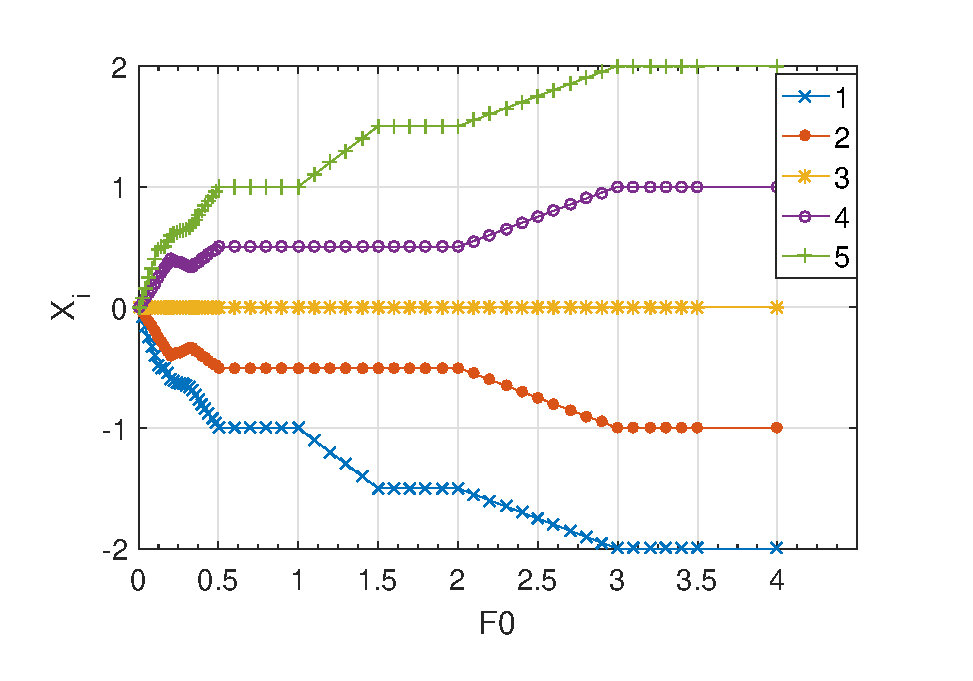
\includegraphics[scale=0.6]{ZhiyuPictures/N=5_GS_pre_2_rev.eps}
\caption{particles' position at ground states }
\label{fig:GS1}
\end{figure}


%\begin{figure}[hbtp]
%\centering
%\includegraphics[scale=0.3]{D:/matlab2016/MolecularDynamics/figure/Eg1.eps}
%\caption{ground state Energy with $F_0$}
%\end{figure}
%\end{comment}

\section{Breathing Frequency}\label{section:breathing frequency}
Usually, to see the response of quantum gas to a quench, one begin simulation with the ground state and then suddenly vary some parameter by a little, for instance, $\omega_0'\rightarrow\omega_0=\omega_0'+\Delta\omega$. In that case, one will observe the radius R oscillating at a certain frequency, which is usually called ``breathing mode".
However, it is quite different in the classical version. Firstly, the ground state may be meaningless. In quantum case, the reason why we care about ground state and low lying excitations is that BEC occur at low temperature. But in classical case, there is no BEC. So it is not necessary to focus on low lying excitations in classical case. Besides, since classical limit is $\hbar\rightarrow 0$, no matter how low the kT is, $\hbar/kT$ is always zero so that classical behavious of low lying excitations is quite different from the quantum one. Secondly, it is no longer necessary to vary parameters ``by a little" in the quench. In quantum case, the small quench $\omega_0'\rightarrow\omega_0=\omega_0'+\Delta\omega$ means the spectrum is shifted slightly, thus one may expect to see some beat phenomenon({\color{red}{?}}). But in classical case, since $\hbar$ vanishes, no matter how small the quench is, one can never recover or proximate the quantum case. Thus it is not necessary to limit ourselves to small quench. 

Furthermore, notice that X and P (normalized) are symmetric for simple harmonic oscillator. In weak interaction limit, the distribution cloud should be circular when the gas is completely thermalized. The difference between thermalized cloud before and after quench is that they are circular under different normalization of phase-space. If we look at both of them in the phase-space normalized according to the final $\omega_0$, we will find shape of the cloud before the quench is an ellipse while the final one is a circle.

Since the number of particles we use in the Molecular Dynamics simulation is limited (usually 5 to 20), the random noise is significant. If we start with a state whose configuration in phase-space is an ellipse slightly deviated from circle, the oscillating amplitude will be too small to be distinguished from noise. Therefore, we start from an extreme case -- line distribution (random x, zero p) and observe the oscillation of R(t). 
\begin{figure}[hbtp]
\center
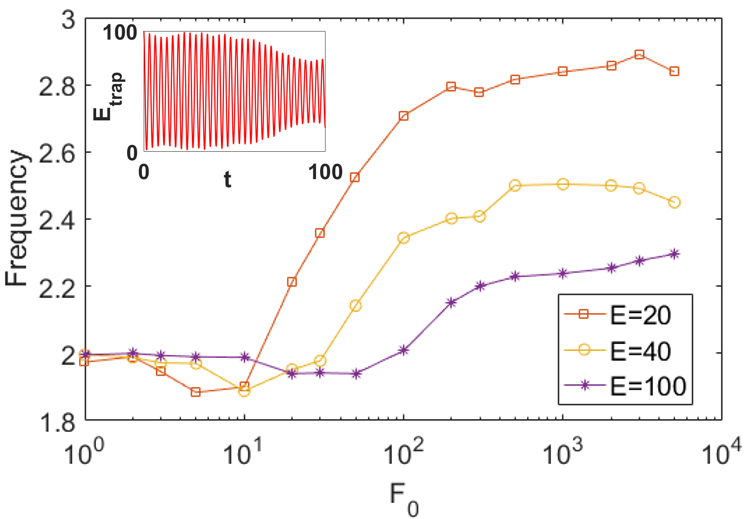
\includegraphics[scale=0.32]{ZhiyuPictures/freq_scanF_differentE_log_2_with_oscillation_demo.png}
\caption{breathing mode frequency measured at different E and $F_0$. Insert: a demonstration of oscillation, $E_{trap}$ is the total potential energy of particles in the trap, which is proportional to $\sum_{is}{x_i^2}$, thus manifest the oscillation behavior of radius R(t) defined in Eq.\ref{eq:def_of_R}. The breathing frequency is measured by taking Fourier transformation of R(t).}
\label{fig:Breathingfrequency1}
\end{figure}

Without interaction, the breathing mode frequency is exactly 2. When there is interaction, the frequency will drift to some other value near 2. We measure the radius of the cloud $R(t)$ and get the frequency spectrum of its oscillation behavior by Fourier transform. Then we take the peak frequency near 2 as the breathing mode frequency. The frequency measured in different E and $F_0$ is shown in the Fig.\ref{fig:Breathingfrequency1}.

The mechanism that deviate breathing frequency from 2 is simple in real space. When two particle bounce, they exchange momentum immediately. It can be interpret as particle A carries its momentum $P_A$ and jump $\sigma$ to the right, while particle B carries its momentum $P_B$ and jump $\sigma$ to the left. In this manner, every collision will save a particle some time $\frac{\sigma}{v}$ . Since $v$ is proportional to R while the number of collision each particle experiences in one period of harmonic oscillation can be estimated by N, we will get $\delta\sim N^{\frac{3}{2}}E^{-\frac{1}{2}}$. 

To see this picture better, let us first introduce a approach to simplify this problem:

\subsection{Rotating frame in Phase-space}
Traditionally, we think of there is a distribution cloud in phase space, and due to harmonic trap, the cloud will rotate at frequency $\omega_0$. When there is interaction, we may think there is a small modification of the frequency $\omega=\omega_0+\delta$. Now we want to understand how $\delta$ is dependent on parameters, so it is better to stand in the rotating frame in the phase space. In this frame, the picture we will see is as follow:\\
\begin{enumerate}[\textbf{*}]
\item All particles are stationary when there is no interaction.
\item The real X and P axis are rotating counter-clockwise, using real X axis to measure distance between particles to determine the interaction at each moment.
\item When there is interaction, particles will gain a ``velocity" in phase space: $\dot{P}=F/m$ . Other effects are all cancelled by frame rotation.
\end{enumerate}


This picture is actually a classical version of the interaction picture. With this picture, we will soon find the dynamic analysis greatly simplified.

In our system, we choose initial velocity to be zero, which means, the particles are aligned on $X|_{t=0}$ axis in phase-space at the beginning. If the breathing frequency of the system is $\omega=\omega_0+\delta$, we will expect to see a line (which may gradually deform into an oval cloud or even an isotropic cloud) rotating at $\delta$ in rotating frame. If we plot x-p with t, we expect to see a spiral motion. Since the motion we see is an additional rotation in rotating frame, we will call it precession. This precession directly leads to the $\delta$.

Fig.\ref{fig:Breathingfrequency2_1} show this precession motion in the rotating frame in phase-space.



\begin{figure*}
\subfigure[$t=0$]{
\begin{minipage}[b]{0.18\linewidth}
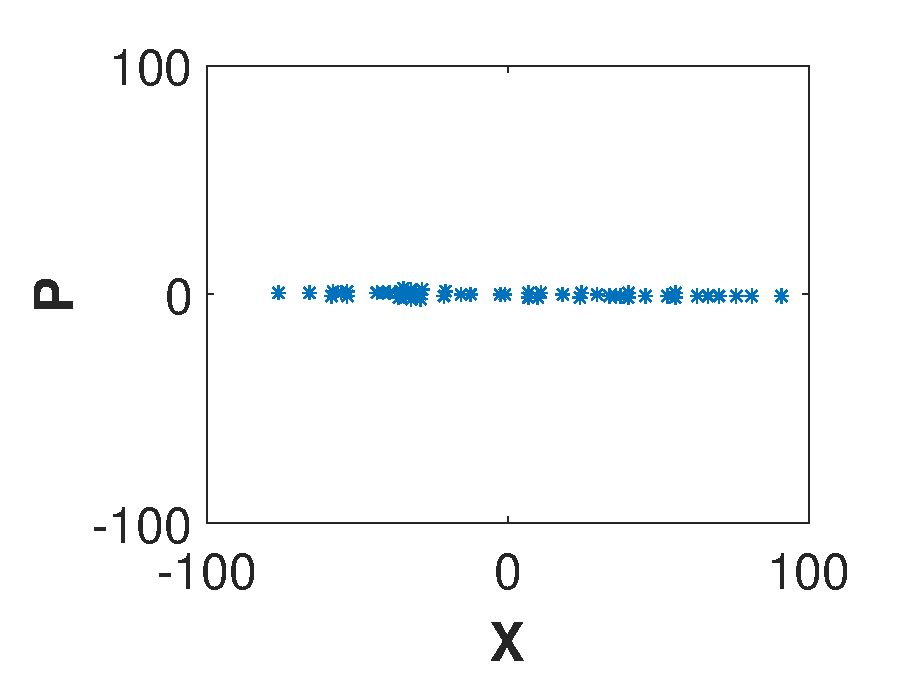
\includegraphics[scale=0.21]{ZhiyuPictures/stationary_frame_t=1-5T_rev.eps} 
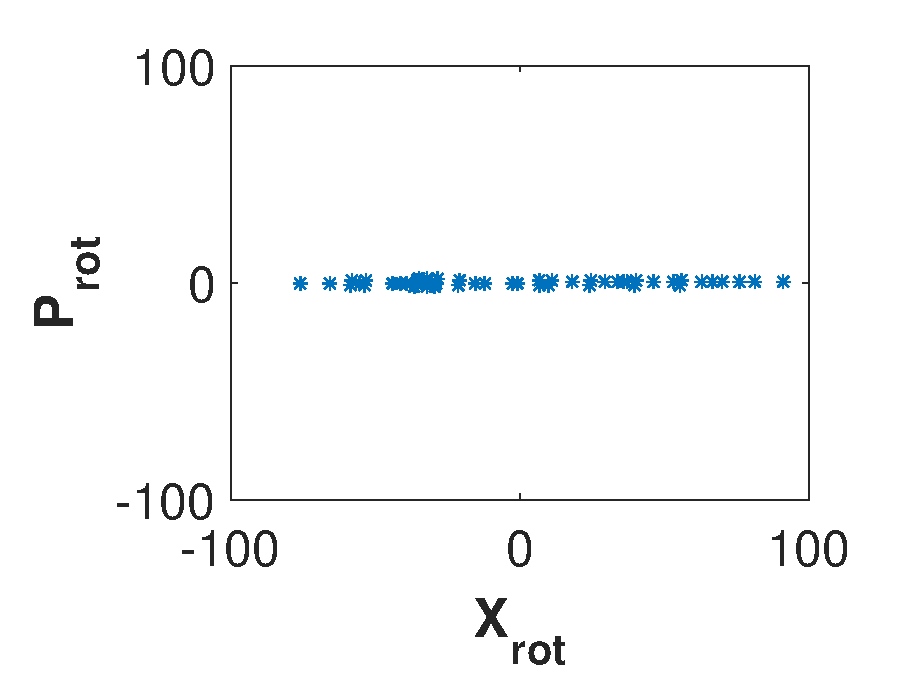
\includegraphics[scale=0.22]{ZhiyuPictures/rotating_frame_t=1-5T_rev.eps}
\end{minipage}
}
\subfigure[$t=\frac{1}{5}T$]{
\begin{minipage}[b]{0.18\linewidth}
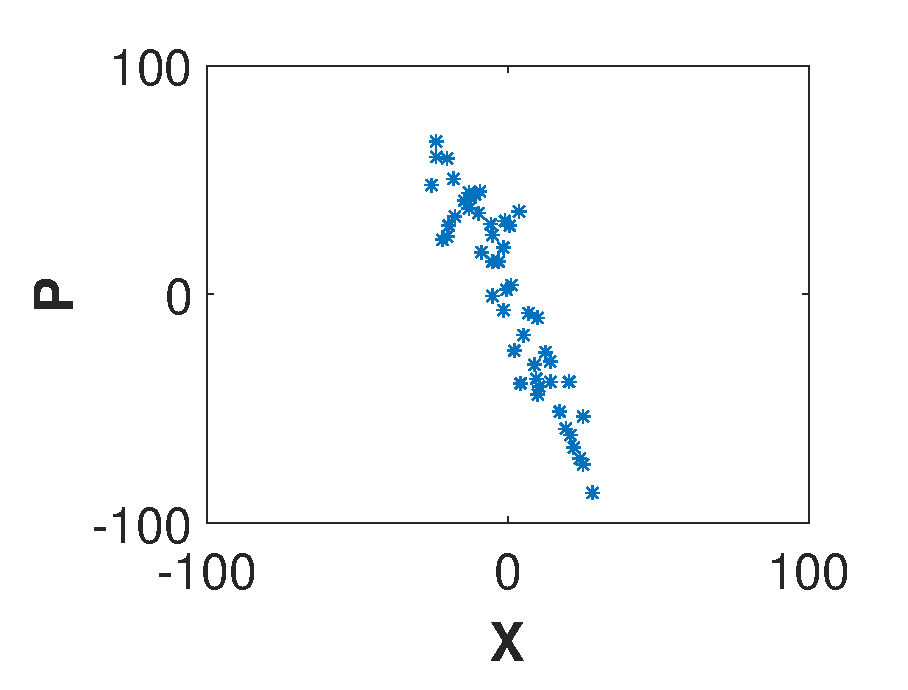
\includegraphics[scale=0.21]{ZhiyuPictures/stationary_frame_t=2-5T_rev.eps} 
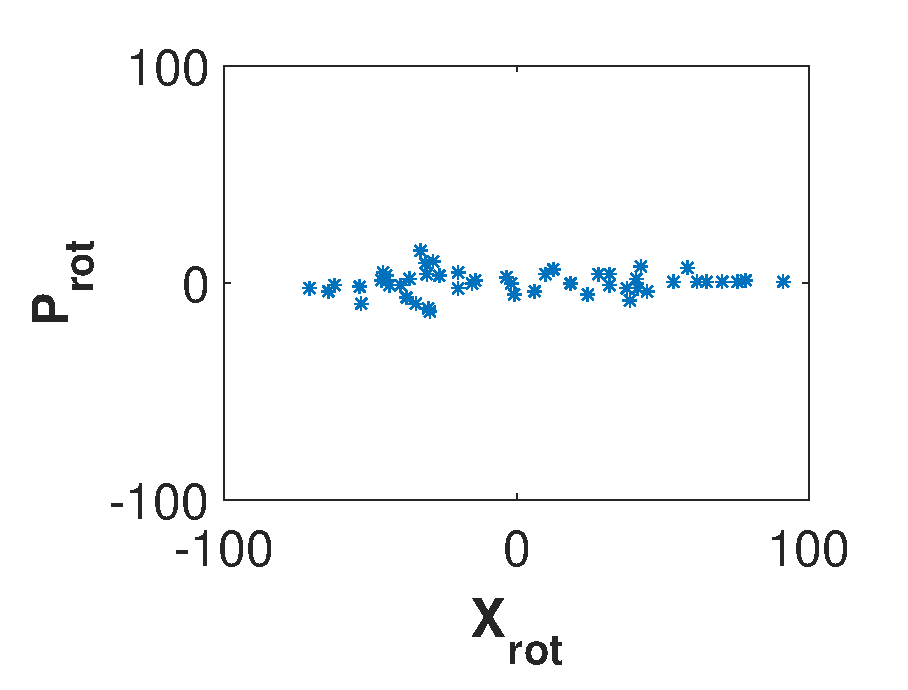
\includegraphics[scale=0.22]{ZhiyuPictures/rotating_frame_t=2-5T_rev.eps}
\end{minipage}
}\subfigure[$t=\frac{2}{5}T$]{
\begin{minipage}[b]{0.18\linewidth}
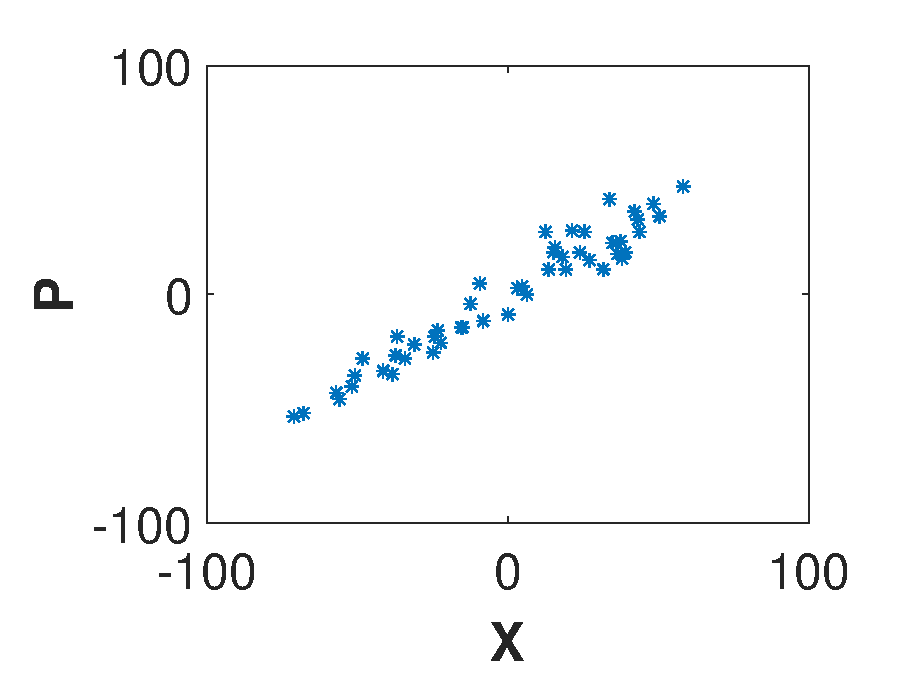
\includegraphics[scale=0.21]{ZhiyuPictures/stationary_frame_t=3-5T_rev.eps} 
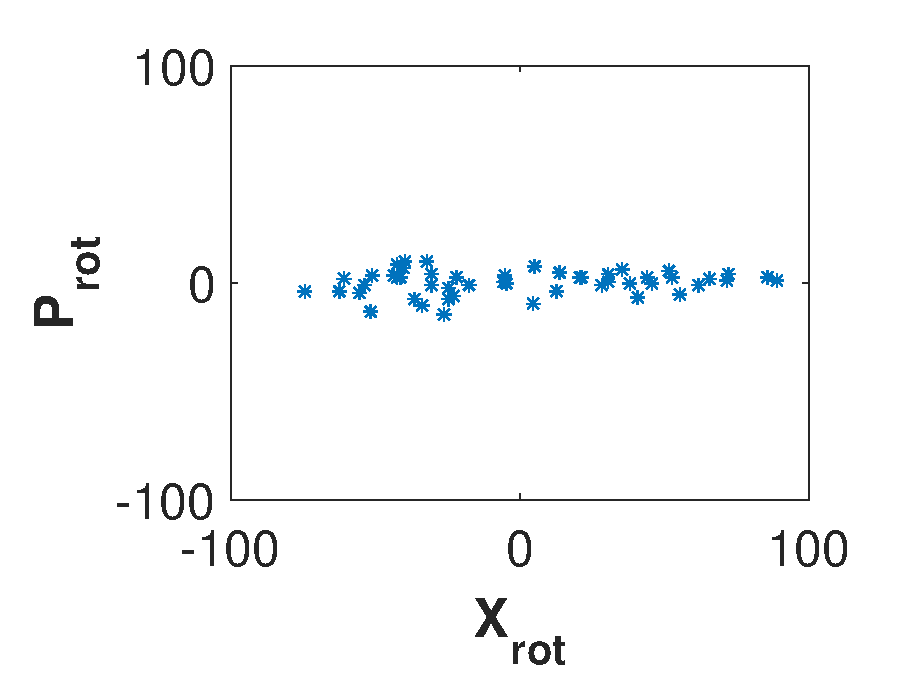
\includegraphics[scale=0.22]{ZhiyuPictures/rotating_frame_t=3-5T_rev.eps}
\end{minipage}
}\subfigure[$t=\frac{3}{5}T$]{
\begin{minipage}[b]{0.18\linewidth}
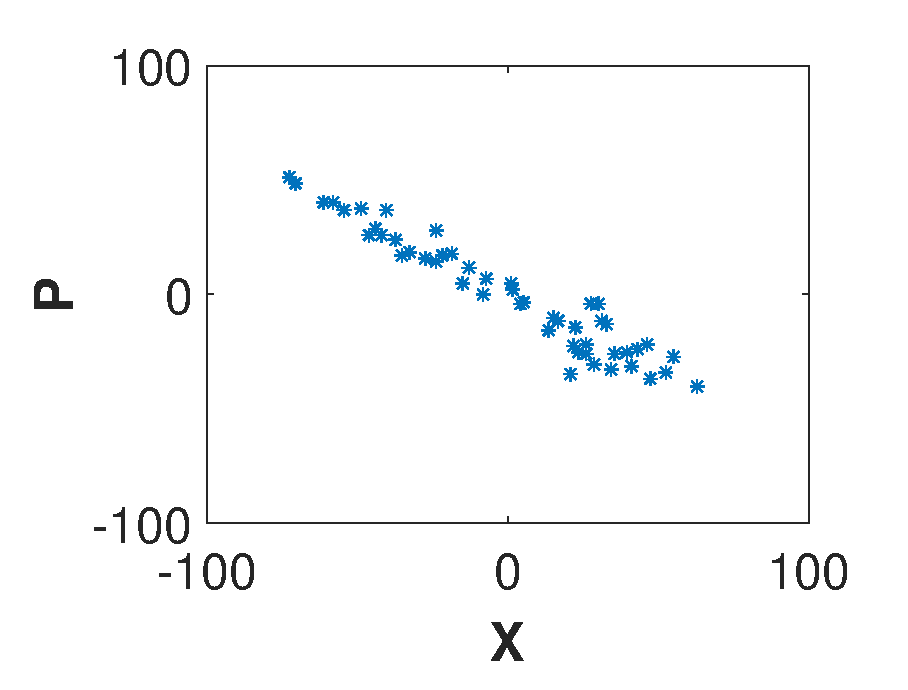
\includegraphics[scale=0.21]{ZhiyuPictures/stationary_frame_t=4-5T_rev.eps} 
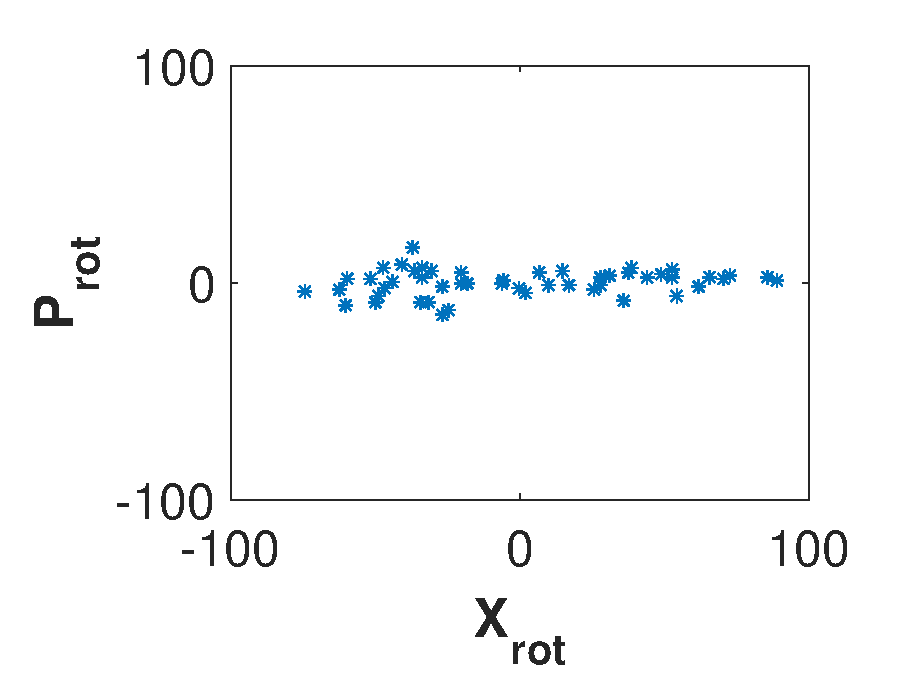
\includegraphics[scale=0.22]{ZhiyuPictures/rotating_frame_t=4-5T_rev.eps}
\end{minipage}
}\subfigure[$t=\frac{4}{5}T$]{
\begin{minipage}[b]{0.18\linewidth}
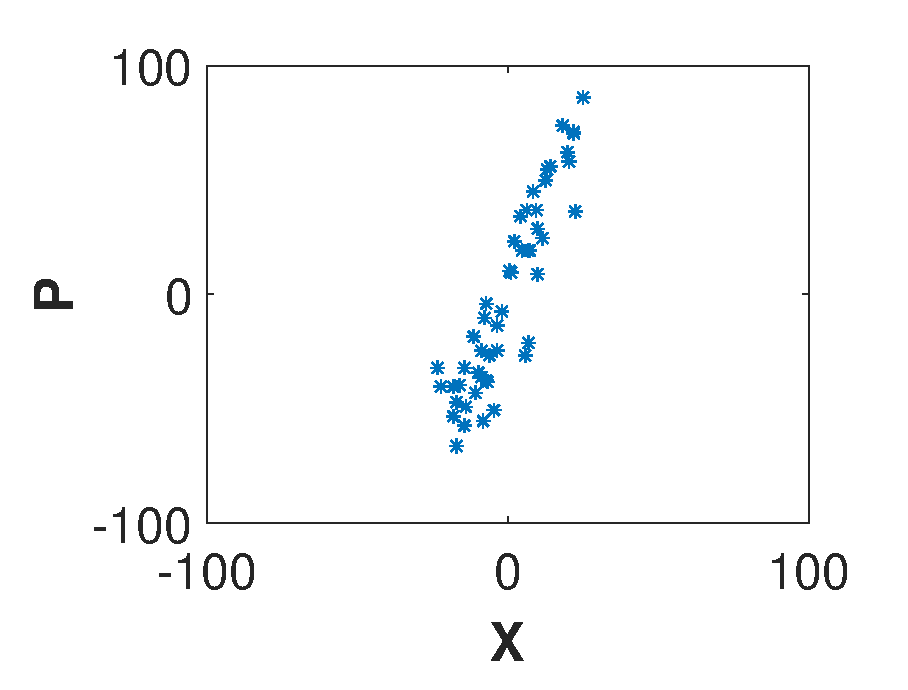
\includegraphics[scale=0.21]{ZhiyuPictures/stationary_frame_t=5-5T_rev.eps} 
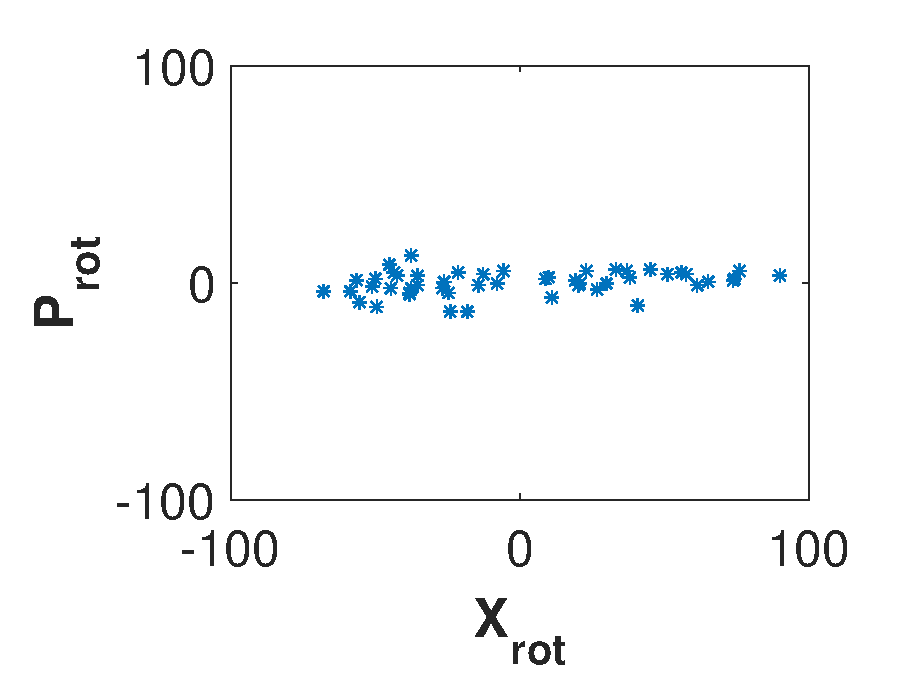
\includegraphics[scale=0.22]{ZhiyuPictures/rotating_frame_t=5-5T_rev.eps}
\end{minipage}
}
\caption{N=50,F0=100,E=50000. Upper(lower) five pictures are snapshot of the configuration of the cloud in the stationary(rotating) frame at t=$\frac{1}{5}T$, $\frac{2}{5}T$, $\frac{3}{5}T$, $\frac{4}{5}T$, $T$ respectively.}
\end{figure*}


\begin{figure*}
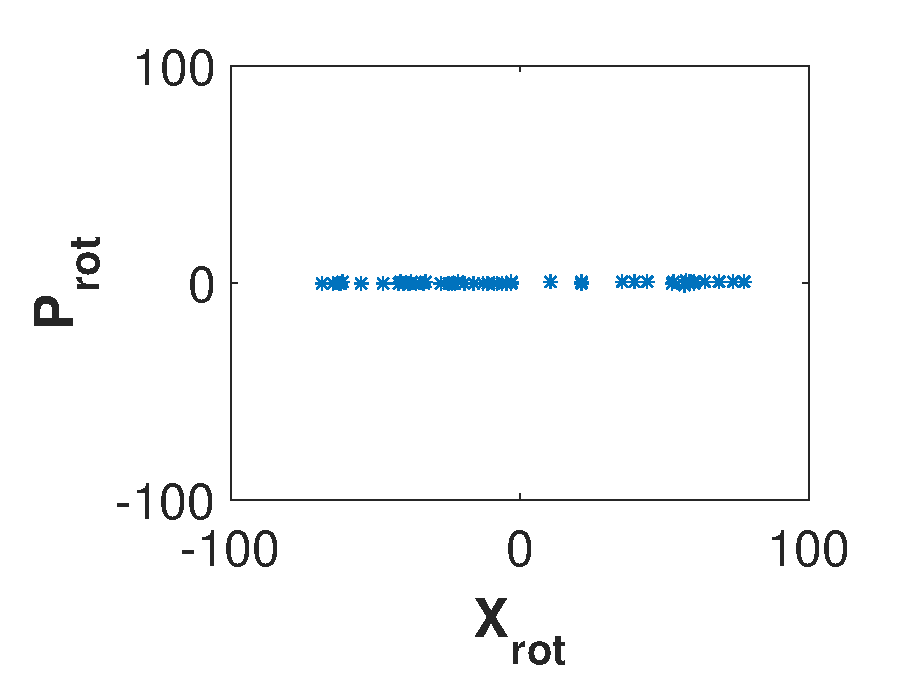
\includegraphics[scale=0.23]{ZhiyuPictures/10_18rotating_frame_t=0T_rev.eps} 
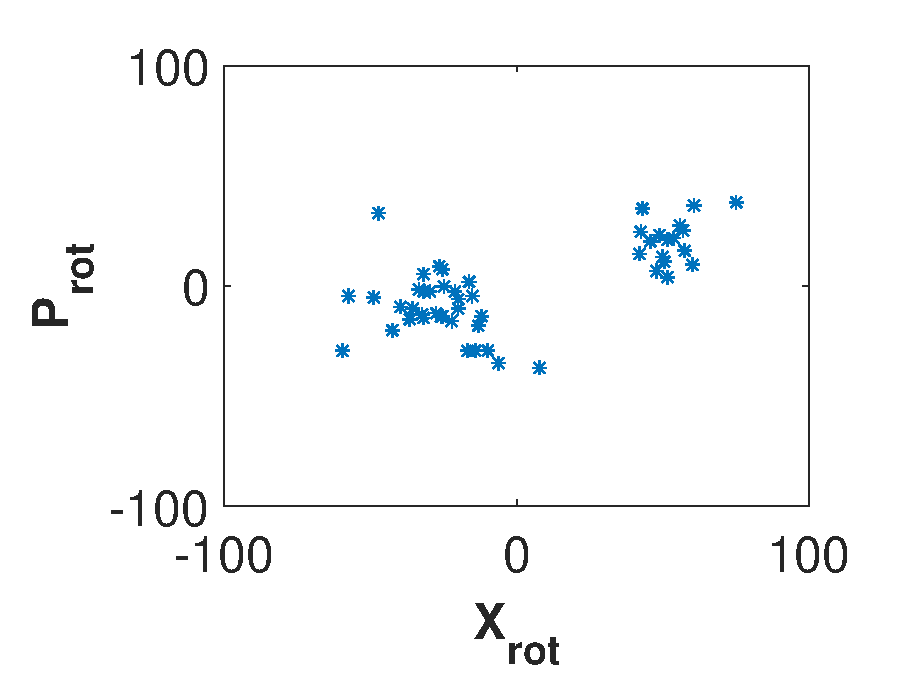
\includegraphics[scale=0.23]{ZhiyuPictures/10_18rotating_frame_t=20T_rev.eps}
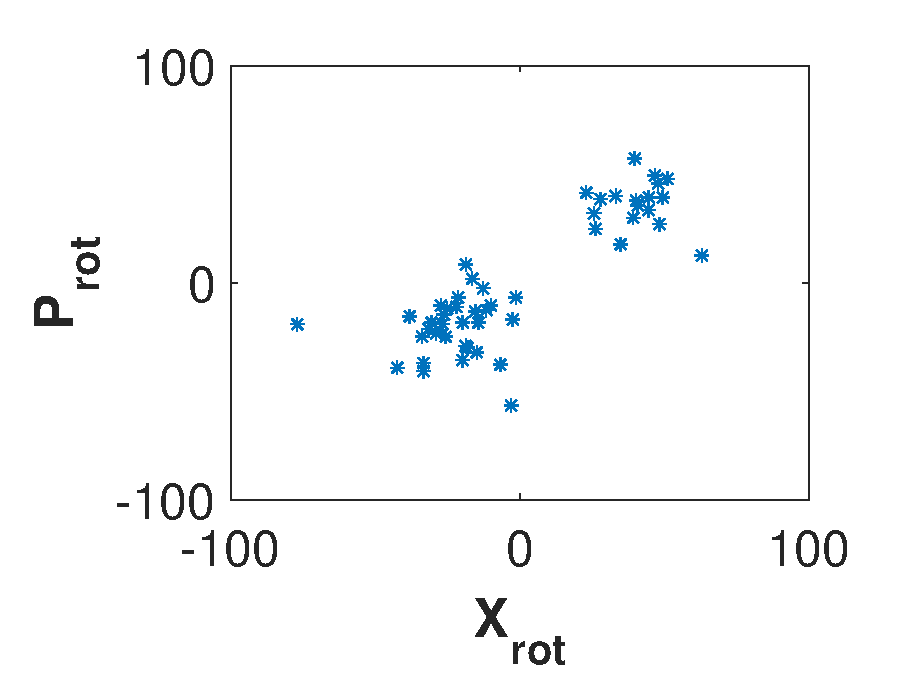
\includegraphics[scale=0.23]{ZhiyuPictures/10_18rotating_frame_t=40T_rev.eps} 
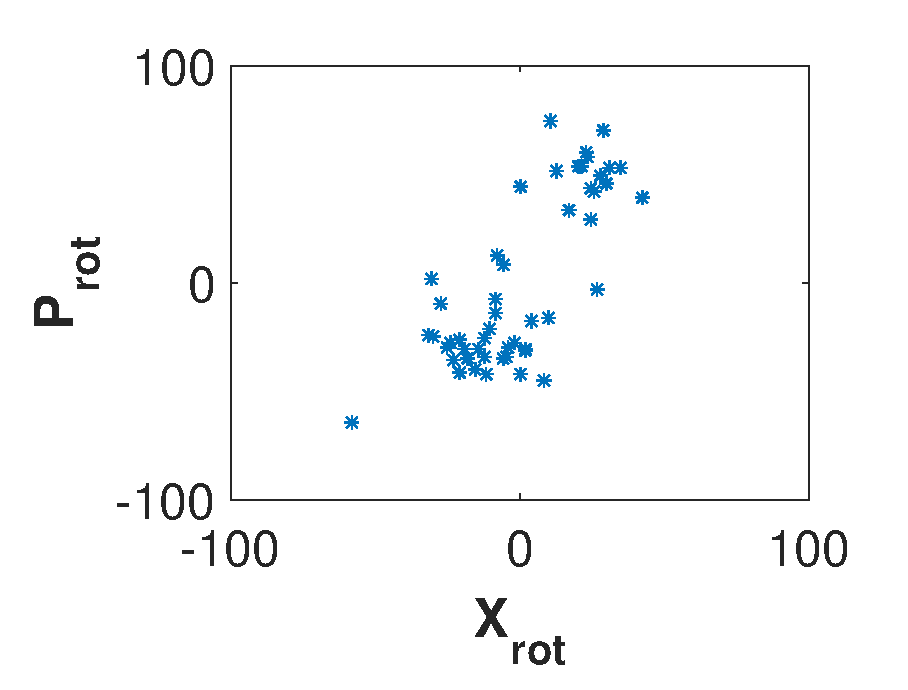
\includegraphics[scale=0.23]{ZhiyuPictures/10_18rotating_frame_t=60T_rev.eps}
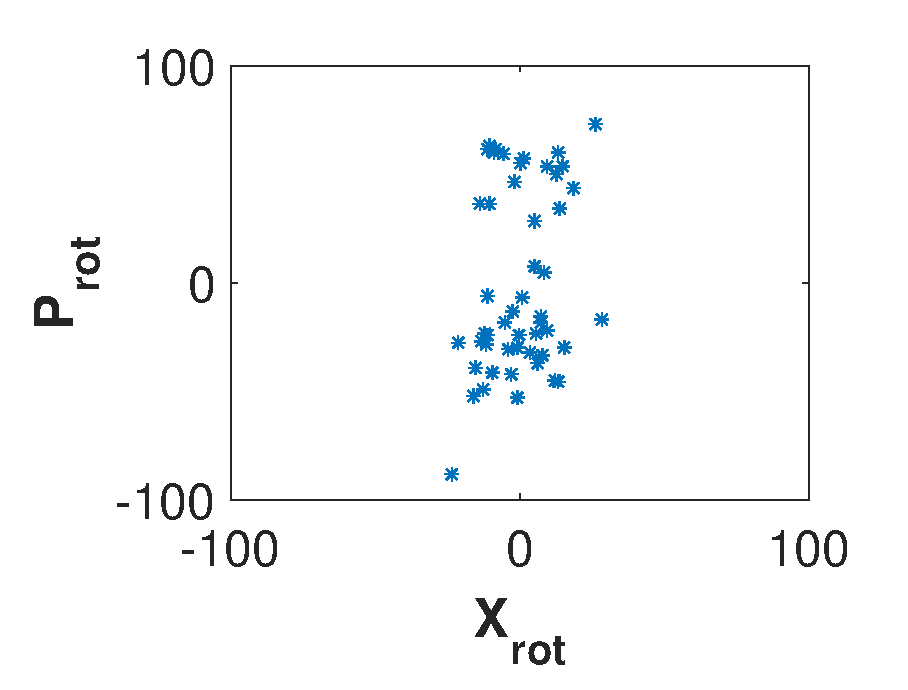
\includegraphics[scale=0.23]{ZhiyuPictures/10_18rotating_frame_t=80T_rev.eps} 
\caption{the precession behavior of cloud viewed in the rotating frame in phase-space. $\frac{t}{T}=0,20,40,60,80$}
\label{fig:Breathingfrequency2_1}
\end{figure*}



\subsection{Estimating Breathing Frequency}
Let us begin with two-particle case. When interaction is very strong, the effect of interaction is equivalent to exchanging momentum when two particles approach each other at distance $\sigma$. In the rotating frame in phase-space, this process can be interpret as follows:

\begin{figure}
\centering
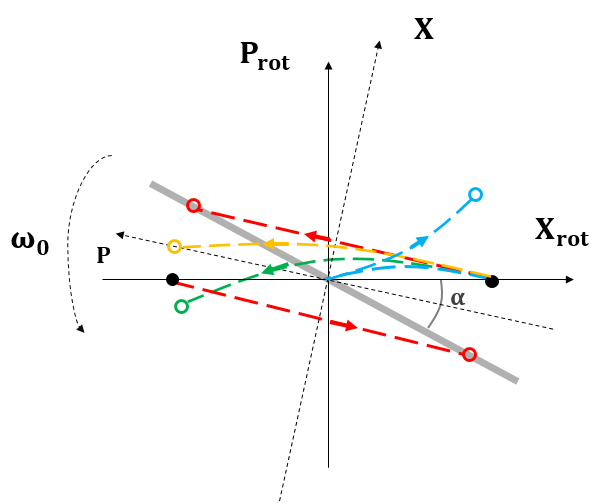
\includegraphics[scale=0.3]{ZhiyuPictures/bounce.png}
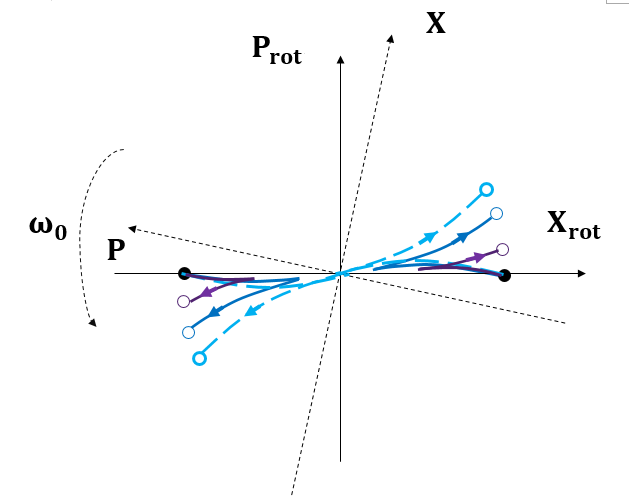
\includegraphics[scale=0.32]{ZhiyuPictures/pass.png}
\caption{a schematic diagram of the collision process: \textbf{(a)}(Upper)when $F_0*\sigma$ is big, particles can not penetrate each other, thus their trajectory in rotating frame is a circular arc.  \textbf{(b)} (Lower) When $F_0*\sigma$ is small, particles easily pass each other, so that the force they feel is not continuous, their trajectory has a turning point(the dashed bright blue trajectory is identical with the one in the upper figure, which is the critical situation between passing and bouncing, that is to say, particles have zero relative velocity when they collide.) }
\label{fig:Breathingfrequency3}
\end{figure}


(See fig.\ref{fig:Breathingfrequency3}(a))Two particles flip to another line(thick gray line) which deviate a small angle $\alpha$ away from original configuration. Similar process happen when there are more particles. In every period of harmonic oscillation, each particle meet N particles and collide 2N times, while half of the collisions (N times) are between particles with huge difference in momentum, which is just the process shown in fig.\ref{fig:Breathingfrequency3}. (As for the remaining half of collisions, colliding particles have small difference in their momentum. Let us say, both particles have positive momentum. In fig.\ref{fig:Breathingfrequency3}, it can be shown that two particles on the same half of the P-axis cannot have strong effect on the rotation of distribution.)

Let us estimate the precession angle $\alpha$ in one collision by $\frac{\sigma}{R}$, which follows from the two-particle case study. Radius of the cloud R can be estimated according to $E=Nm\omega_0^2R^2$
We will get the precession angular velocity 
\begin{equation}
\delta=2\omega_0\frac{N^\frac{3}{2}m^{\frac{1}{2}}E^{-\frac{1}{2}}\sigma\omega_0}{2\pi}
\label{eq:breathingfrequency1}
\end{equation}





When $F_0$ is not that large, the frequency behavior seems complicated (see fig.\ref{fig:Breathingfrequency1}). Usually, when $F_0$ increase, frequency goes down below 2 first and then rise up and converge to some value higher than 2. The reason could also be well understood with the mechanism described before. In the former discussion, we goes to high $F_0$ limit, which means particles exchange momentum in infinitesimal time. For $F_0$ is not very big, the finite interaction time should be taken into consideration. During this time, the behavior of each particle in phase space is exactly moving along the direction of the real P axis at 'velocity' $F0/m$. Since the real P axis is rotating counter-clockwise, the particle will follow the circular trajectory(orange and green dashed line in fig.\ref{fig:Breathingfrequency3}) the $\alpha$ that we once use to estimate the precession motion should decrease with the increase of interaction time. There should be some ``critical point" where $\alpha$ goes from plus to minus (dashed green line). At this point, we will see the precession stop so that the frequency is 2. 


\begin{figure}
\centering
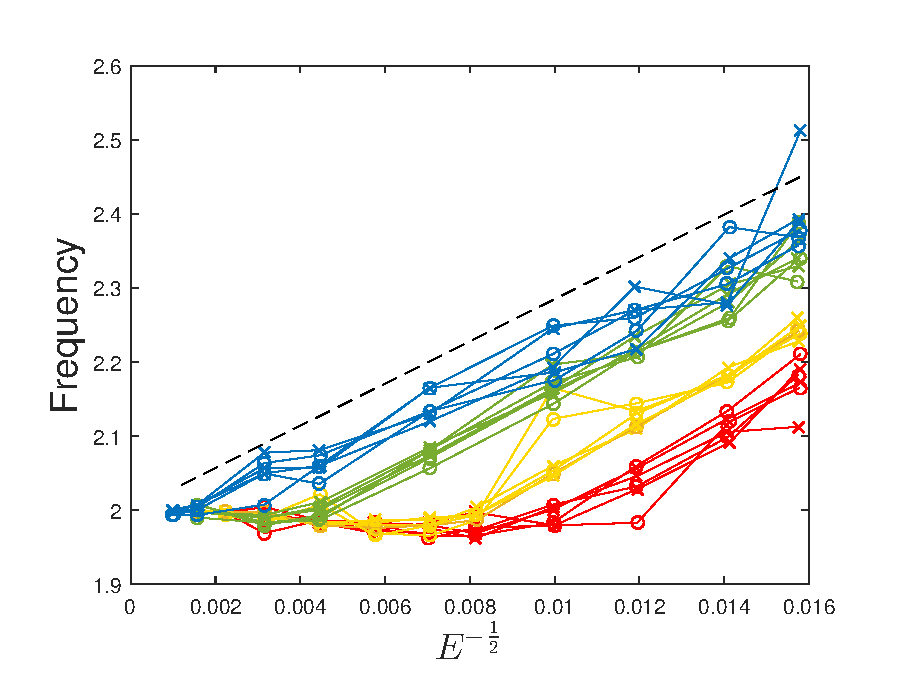
\includegraphics[scale=0.6]{ZhiyuPictures/freq_scanF_scanE_pre.eps}
\caption{dependence of breathing frequency on Energy, N=20. Different color stands for different $F_0$: {\color{red}{Red}} for $F_0$=2000; {\color{yellow}{Yellow}} for $F_0$=3000; {\color{green}{Green}} for $F_0$=10000;  {\color{blue}{Blue}} for $F_0$=100000. Run with 3 different initial states in each case, and in each run, measure the frequency in 0-100 time unit(label as crosses) and in 900-1000 time unit (label as circles). The black dashed line is the prediction of Eq.\ref{eq:breathingfrequency1}.}
\label{fig:Breathingfrequency4}
\end{figure}

The dependence of frequency on energy and $F_0$ is shown in fig.\ref{fig:Breathingfrequency4}. For the first thing, as expected when $F_0$ is high the frequency behavior is well-described by linear prediction Eq.\ref{eq:breathingfrequency1}. Secondly, the figure shows the frequency's dependence on $F_0$. As we explained, when $F_0$ is not so large, the precession angle decrease. In language of real space, the finite $F_0$ create a finite approaching time, thus consumes the time saved by finite-range collision. As a result, the frequency should be lower when $F_0$ decrease, and reach 2 earlier.

the critical point that frequency falls to 2 can be estimate by:
\begin{equation}
\omega_0 \tau=\alpha
\end{equation}
which states that the approaching time $\tau$ exactly cancels the precession angle derived before
$\tau$ can be estimated by $R/F_0$. With some math, one can show that this condition is equivalent to 

\begin{equation}
\frac{E}{N}=F_0\sigma
\end{equation}
which is the same as the criterion of whether two particle will bounce or pass by if one estimate the average internal energy of a pair with $\frac{E}{N}$. This argument indicate the reason why we see frequency stop falling down below 2 as one should expect with previous discussion:\
All our previous analysis based on fig.\ref{fig:Breathingfrequency3} only studies the case of bouncing. If the energy of particles are so large that they often overcome the interaction potential barrier and pass each other, the situation would be completely different. In that case, in fig.\ref{fig:Breathingfrequency3}, particles will move a little bit out of their initial position, and soon move back, almost return to their initial place. In this manner, the interaction do not affect the distribution of the cloud in phase space. Thus, the frequency will stay near 2 when E is large.

Before completing the discussion, it is necessary to point out that none of the argument here require ``energy thermalization". In addition, if the system is completely thermalized in terms of their phase of orbit in phase space, the argument will no longer work -- there is a stable isotropic distribution in phase space, no matter how the cloud rotate, no oscillation can be observed.


\section{Thermalization}\label{section:Thermalization}
\subsection{Dynamics Study}
It is natural to think that a many-body system with interaction will be thermalized in ``usual" case. To study the condition of thermalization is equivalent to find out the mechanism that prohibits the system from ergodic. We begin the study with two-particle motion. 
\subsubsection{two particles}

\begin{figure}[hbtp]
\centering
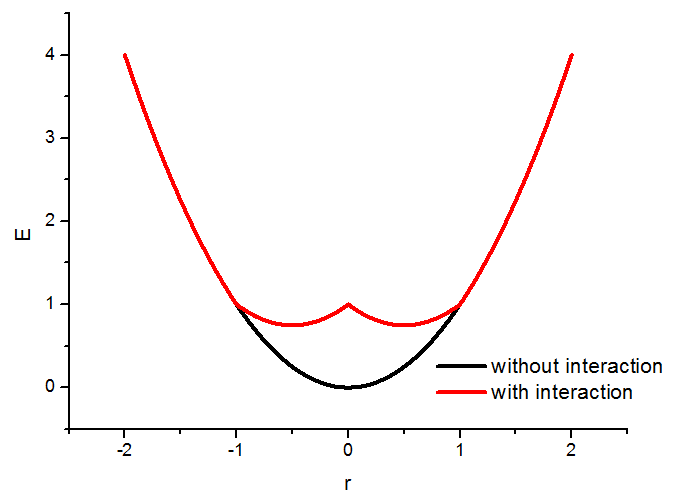
\includegraphics[scale=0.2]{ZhiyuPictures/effective_potential.png}
\caption{effective potential for two-particle system}
\label{fig:thermalization2}
\end{figure}

To see the way interaction change the orbit (energy level) of the particles, we had better start from two-particle case.

We can always think of them in the reference frame of their center of mass ``C". In frame C, one can easily show that when there is no interaction what we will see is that two particles are bound together by a harmonic trap center at C (black line in fig.\ref{fig:thermalization2}). So their relative motion is also a harmonic oscillation. 

In this case, the system has two frequency components. The first one is the frequency of C, which is just $\omega_0$ . The other one is the frequency of their relative motion $\omega_r$, which is slightly deviated from $\omega_0$. The deviation grows with the increase of $F_0$ and the decrease of internal energy of the pair. As a result, when the $F_0$ is small and when the E is large, a beat with low frequency $\omega_r-\omega_0=\delta$ will exist. This phenomenon means energy transfer between particles are inefficient, thus it will slow down the thermalization process. 



\begin{figure}

\subfigure[$E_i=2$]{
\begin{minipage}[b]{0.22\textwidth}
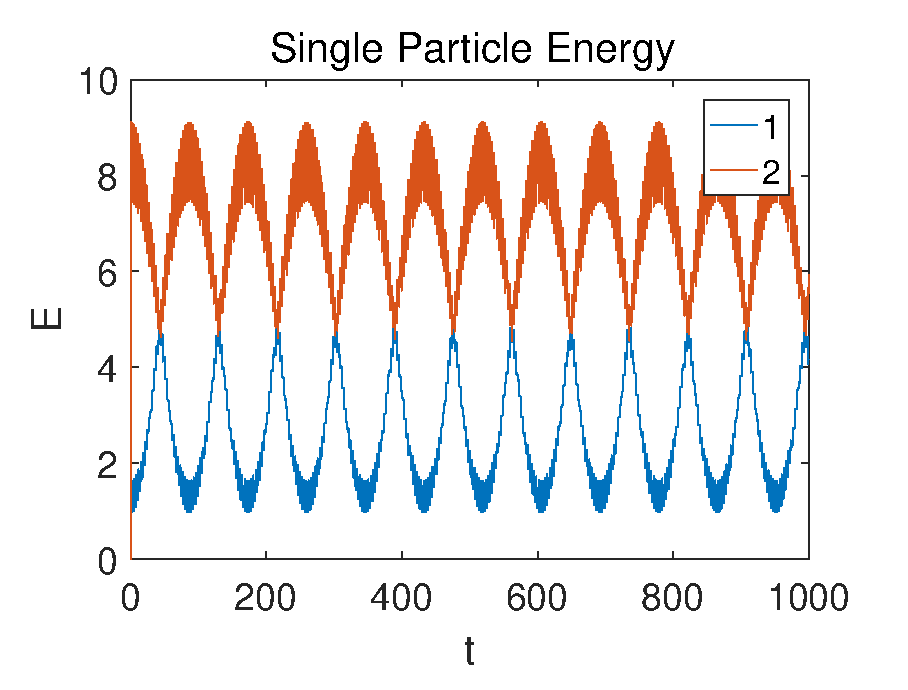
\includegraphics[scale=0.3]{ZhiyuPictures/10_23_N=2_F0=1_Er=2_single_particle_energy_pre.eps} 
%\includegraphics[scale=0.2]{ZhiyuPictures/twoparticle_Er=2_phasespace.eps}
\end{minipage}
}
\subfigure[$E_i=3$]{
\begin{minipage}[b]{0.22\textwidth}
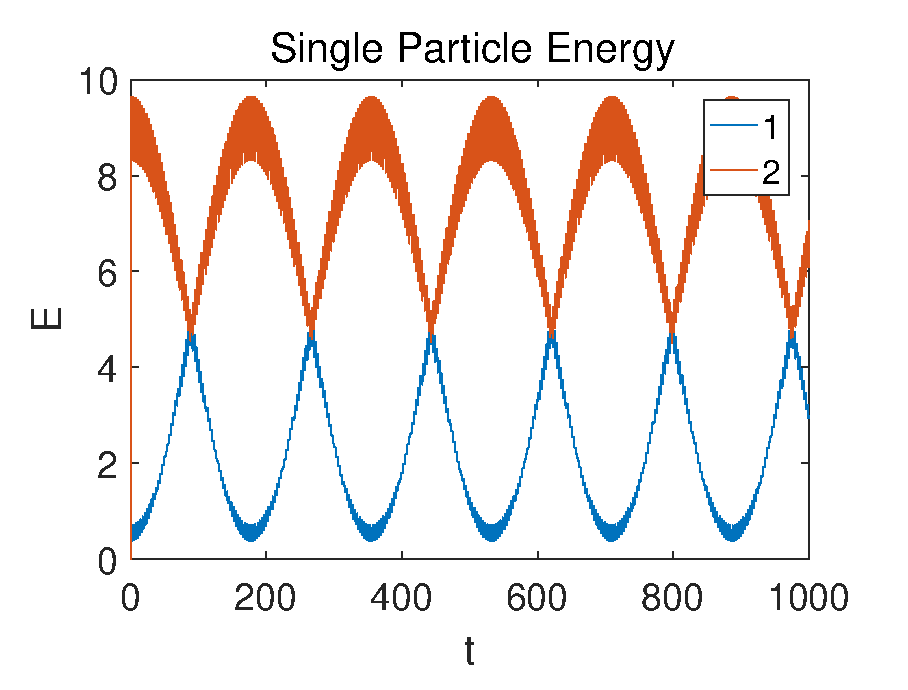
\includegraphics[scale=0.3]{ZhiyuPictures/10_23_N=2_F0=1_Er=3_single_particle_energy_pre.eps} 
%\includegraphics[scale=0.2]{ZhiyuPictures/twoparticle_Er=3_phasespace.eps}
\end{minipage}
}
\subfigure[$E_i=5$]{
\begin{minipage}[b]{0.22\textwidth}
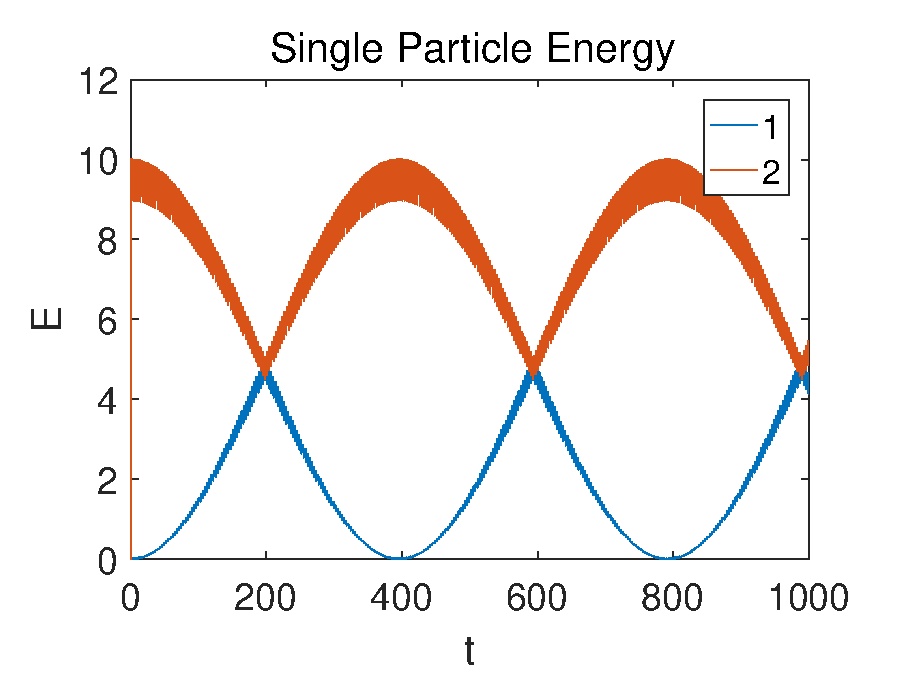
\includegraphics[scale=0.3]{ZhiyuPictures/10_23_N=2_F0=1_Er=5_single_particle_energy_pre.eps} 
%\includegraphics[scale=0.2]{ZhiyuPictures/twoparticle_Er=5_phasespace.eps}
\end{minipage}
}
\subfigure[$E_i=10$]{
\begin{minipage}[b]{0.22\textwidth}
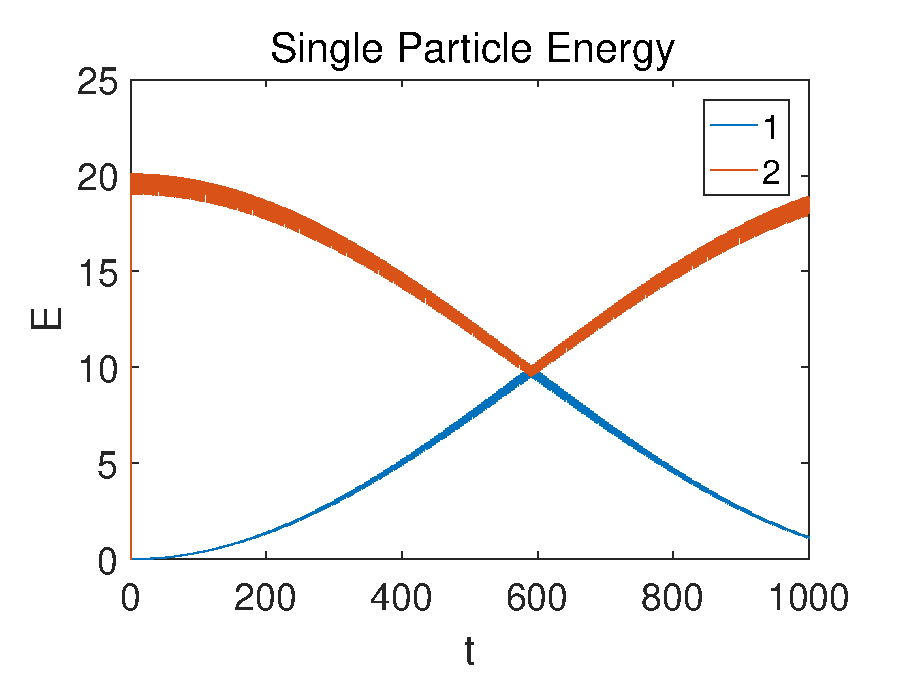
\includegraphics[scale=0.3]{ZhiyuPictures/10_23_N=2_F0=1_Er=10_single_particle_energy_pre.eps} 
%\includegraphics[scale=0.2]{ZhiyuPictures/twoparticle_Er=10_phasespace.eps}
\end{minipage}
}

\caption{the dependence of beat frequency on internal energy. The diagram is the energy of two particles. Here, $F_0$ is set to be 1. In this case, the larger $E_i$ is, the lower the beat frequency is. \label{fig:thermalization1}}%Actually in very low energy, we can retrieve a beat, but that is for different reason -- it is a beat between $\omega_0$ and $\frac{\omega_0}{2}+\delta $ 

\end{figure}




\subsubsection{More particles}
Now let's consider the three-particle case. For two particle, the motion is non-chaotic. On the other hand, intuitively, we will say that three-body motion is chaotic so that the system could be ``thermalized" soon. However, in some cases, the time scale of thermalizing could still be very long. Suppose two of them, say, A and B, has small internal energy, which means their distance and relative velocity are both small. Meanwhile, suppose particle C has some energy quite different from A \& B. In this case, A \& B will often be in the interaction, while C will pass both of them at a high speed in each period. How will energy transfer between C and the two-particle system A and B? Since the relative velocity of C and the two-particle system is usually large, C will pass A-B pair in a short time $\tau\sim\frac{\sigma}{R}$ ($\tau\ll\frac{2\pi}{\omega}$). C gives A a push when approaching it, and then push A back when leaving.  As has been discussed in the two-particle case, this process is equivalent to giving A a very small velocity ($\sim O(\frac{\sigma}{R})$) in the background of a trap. Since both the position and velocity of A and B are close($|x_A-x_B|\sim\sigma$), the velocity increase of A \& B are almost the same (difference$\sim O(\frac{\sigma^2}{R^2})$). In this manner, the passing of particle C only kicks the center of mass of the A-B pair slightly, leaving the internal motion of the pair unaffected. In another word, the existence of C will not have significant effect on the energy transfer between A and B, but only ``dance" with their center of mass. The physics of the ``dance" is similar to the dance between two particle. As is shown in fig.\ref{fig:thermalization4}, the particles with energy close to each other tends to form a pair with small internal energy and the pair's internal energy transfer is relatively stable.

\begin{figure}
\centering
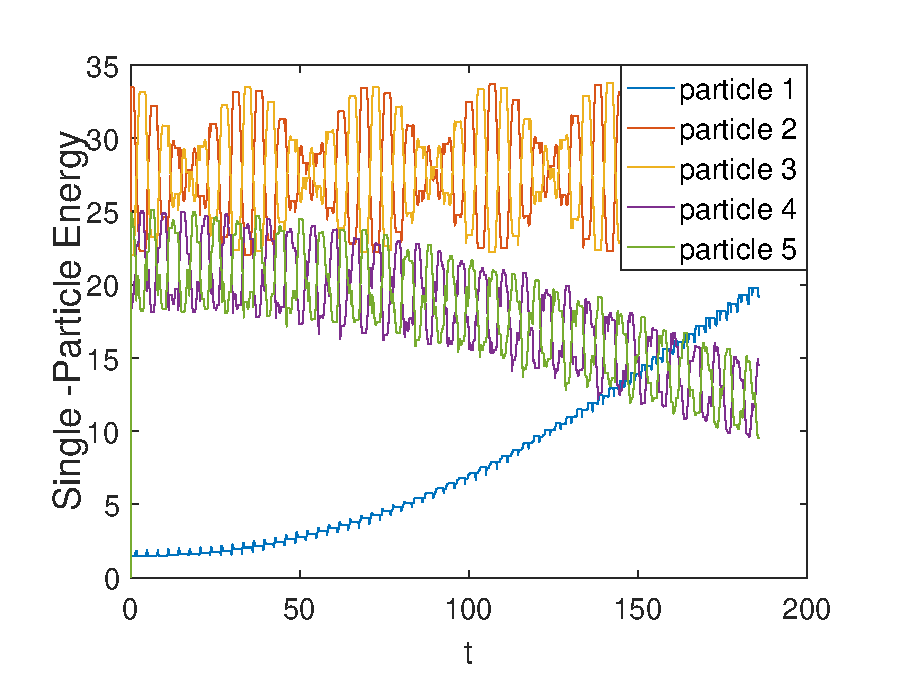
\includegraphics[scale=0.5]{ZhiyuPictures/pair1_pre.eps}
\caption{evolution of single-particle energy}
\label{fig:thermalization4}
\end{figure}

The argument above still holds in many-particle case. Once we start from some configuration where n particles have a set of close energy levels $\left\lbrace E_n\right\rbrace $ and another m particles have another set of energy levels close to each other $\left\lbrace E_m\right\rbrace $, and $\left\lbrace E_n\right\rbrace $ is quite different from $\left\lbrace E_n\right\rbrace $, we will find these two systems oscillating on the energy level diagram at low frequency. 
The discussion above gives us some pictures about the non-ergodic state. For these state, life time is rather long so that once the system reach such configuration (or certain energy distribution), it will take a long time(more than $10^4$ periods for N=5 case) to decay. 

\subsection{Thermalization condition}
The main obstruct to get an thermalized state (which can be examined by observing distribution) is the low frequency oscillation mentioned before. Because once these modes are excited, the relaxing time could be very long($\textgreater 10^4$). As a result, to achieve ergodic state, we have to avoid such low frequency oscillation. According to our discussion before, the solution is to make internal energy of each two-particle pair not ``too large". Though it is impossible to express the internal energy of every pair in terms of the total energy $E$, we can estimate it by the average energy, which is $\frac{E}{N}$. At least they are of the same order. The thermalization condition could be given by:
\begin{equation}
F_0\sigma\sim\frac{E}{N}
\label{eq:thermalizatiton condition}
\end{equation}



\begin{figure}[hbtp]
\centering
%\includegraphics[scale=0.2]{ZhiyuPictures/distribution1_scanF0_E=100_3.eps}
%\caption{Distribution scan $F_0$, $E=100$, $N=5$, $\sigma=1$ {\color{red}{Run again!}} }
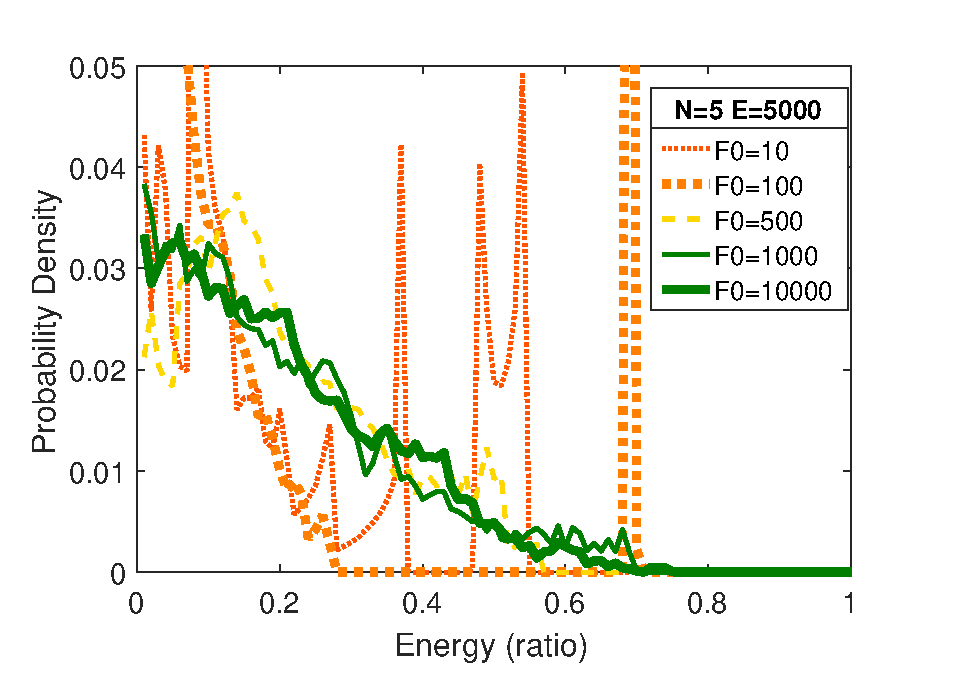
\includegraphics[scale=0.5]{ZhiyuPictures/N=5_energydistribution_pre_rev1.eps} 
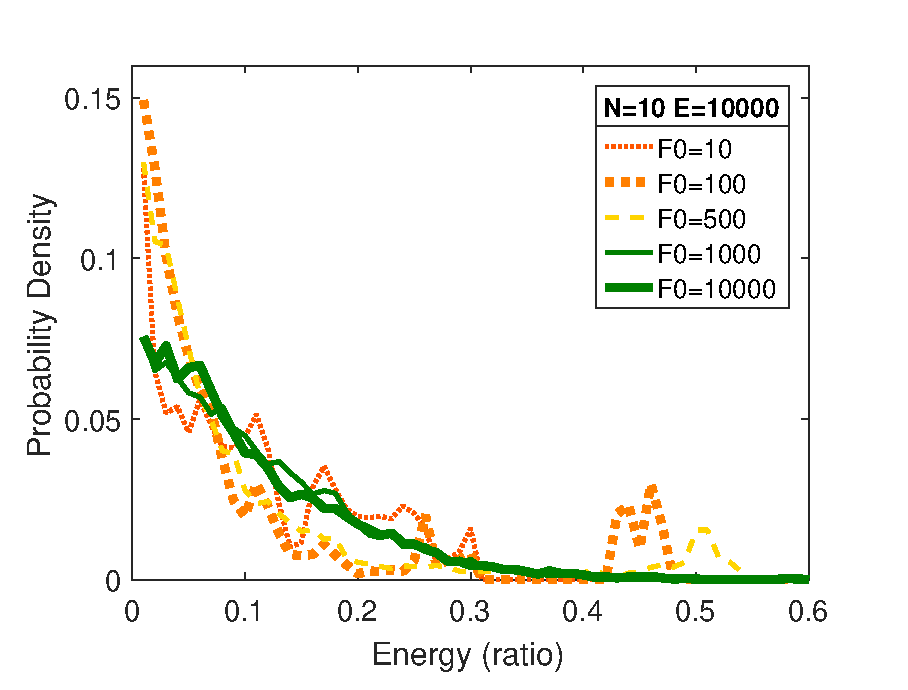
\includegraphics[scale=0.5]{ZhiyuPictures/N=10_energydistribution_pre_rev1.eps}
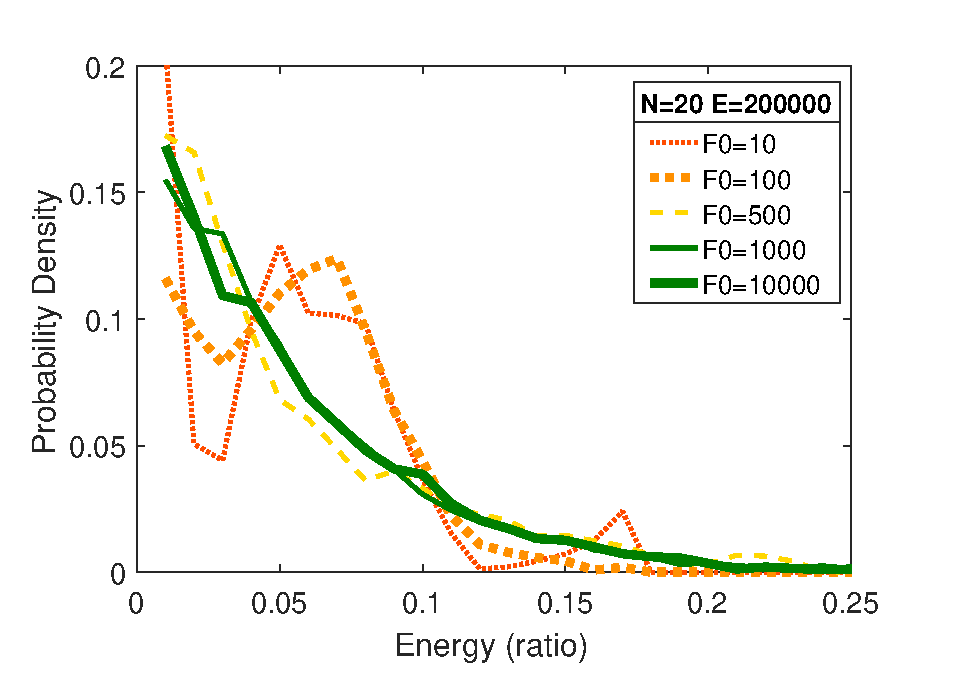
\includegraphics[scale=0.5]{ZhiyuPictures/N=20_energydistribution_pre_rev1.eps}
\caption{the energy distribution measured in $\sim 10000$ time units, as will be verified later, {\color{green}{green}} curves corresponds to Boltzmann distribution; {\color{red}{red}} curves are obviously non-Boltzmann, while the {\color{yellow}{yellow}} ones are intermediate case, represent ``thermalization threshold". In three figures for different N, we choose E/N identical (=1000), and thermalization is reached at $F_0=500$-$F_0=1000$, which is consistent with our prediction in Eq.\ref{eq:thermalizatiton condition}}
\label{fig:thermalization5}

\end{figure}

\begin{figure}
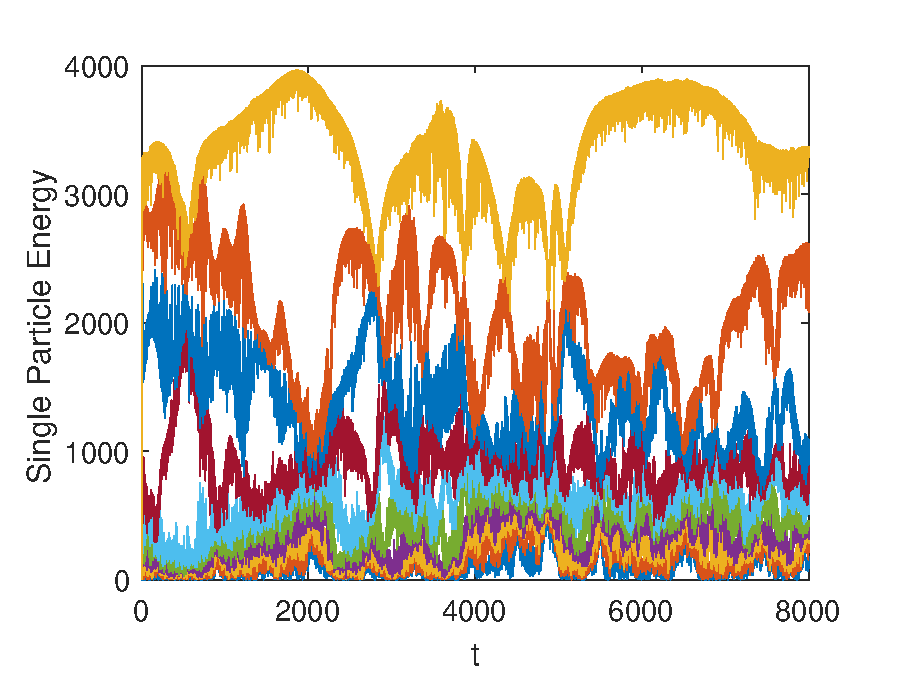
\includegraphics[scale=0.6]{ZhiyuPictures/10_23_N=10_single_particle_energy_F0=200_pre.eps} 
\caption{energy of each particle, $F_0=200$}
\label{fig:thermalization6}

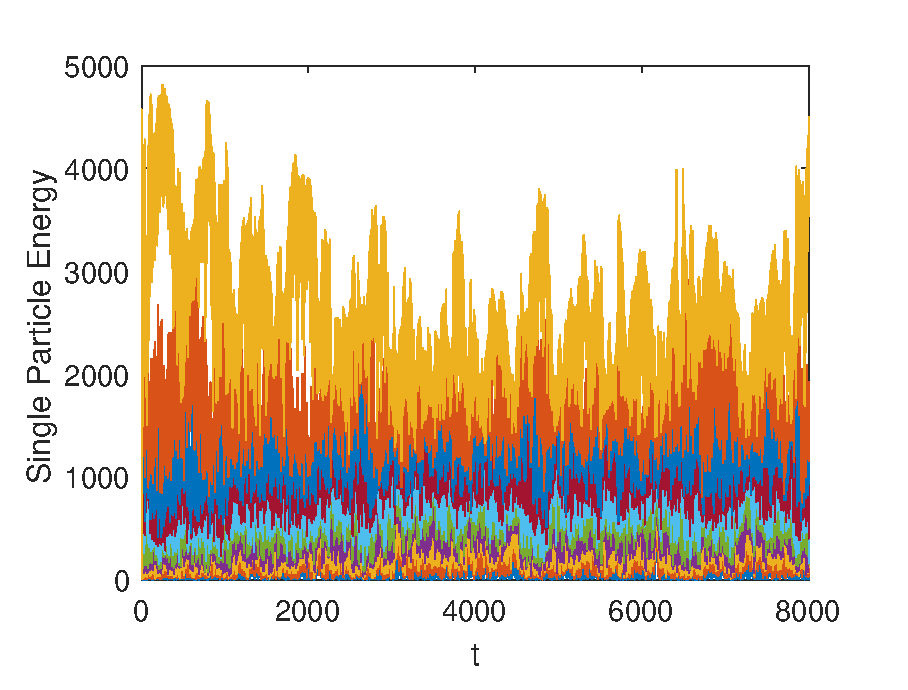
\includegraphics[scale=0.6]{ZhiyuPictures/10_23_N=10_single_particle_energy_F0=1000_pre.eps} 
\caption{energy of each particle, $F_0=1000$}
\label{fig:thermalization7}
\end{figure}

As is shown in fig.\ref{fig:thermalization5} above, the critical point for reaching ``Boltzmann-like" distribution (later we will verify that it is Boltzmann distribution) is $F_0=500$-$F_0=1000$ (we always set $\sigma=1$), while the average energy $\sim 1000$, as we expected, they are of the same order. As a supplementary proof of our argument, fig.\ref{fig:thermalization6} and fig.\ref{fig:thermalization7} show the great difference of single-particle energy between two examples of below and above the thermalization threshold ($F_0=200$ $\&$ $F_0=1000$ for $N=10, E=10000$): in the former one there is always some particle maintained at high excitation, while in the latter the system probably goes to ergodic. To date, we have verified that the threshold of thermalization, which is $\frac{NF_0\sigma}{E}\sim1 $ , and corresponding feature of their energy distribution in two side of the threshold.

One may think that this condition only means that the energy transfer in every collision is much smaller than the energy interval. But this is not the whole story. The essential difference between these two regime lies in whether the energy transfer in every collision is correlated: In thermalizable regime, the energy transfer in every collision is much smaller than the energy interval, which definitely slows down the energy transfer. What is more, because of this, the particles is less interfered by other particles so that two-particle analysis survives. It means that for a particle pair, the energy transferred in this collision is correlated with the one in the next time. In this manner, each particle in the pair will pick up some energy in several collisions, and then return it back to its partner -- which is just what the long term beat effect tells us. Thus the particles energy is localized in certain value. On the contrary, if we go to non-thermalizable regime, the energy transfer is so fast that for each particle don't remember their partners. As a result, the energy transferred in every collision between two particles are no longer correlated, which is equivalent to say that two-particle analysis breaks down. Instead, the energy transfer is completely random, with a non-zero amplitude. On the single-particle energy diagram, what we expected to see is a ``one dimensional random walk" ,so energy levels quickly spread around the diagram.

To sum up, the thermalization threshold not only tells us whether the amplitude of energy transfer in every collision is small enough compared to particles' energy, but also shows whether the ``correlation time" of particle pair is much longer than the characteristic time of the system (the oscillation period).  


\subsection{Verifying Boltzmann distribution}
Thermalization could have different definition. In our system, the ``thermalization" we want to find means ``losing all the memory of initial state". One of the most important information of initial state is energy distribution. 
 
For an isothermal system, the energy distribution of the whole system follows the Boltzmann distribution in equilibrium state. However, to our knowledge, there is not any obvious conclusion about the distribution for an isolated system where the total energy is conserved.

But intuitively, one will expect that if we measure the energy of a subsystem, e.g. one particle, then we will get a Boltzmann distribution because the rest part of the system serves as a bath for this particle. The temperature of this isolated system is defined according to $Nk_BT=E$. It is evident that this argument only hold when the energy of the single particle is not too big --- if one particle take up 50\% of the total energy, the rest could no longer be thought of as a good bath.

In the first picture below, we verify this argument by measuring the energy distribution of every particle at N=10 for different F0 at E=1000 (parameters here satisfy thermalizing condition). In the other two, we tested different N.


\begin{figure}[hbtp]
\centering
%\includegraphics[scale=0.5]{ZhiyuPictures/distribution_at_N=5_F0=10000_pre.eps}
%\caption{Energy distribution, N=5, F0=10000}
%\label{fig:thermalization8}

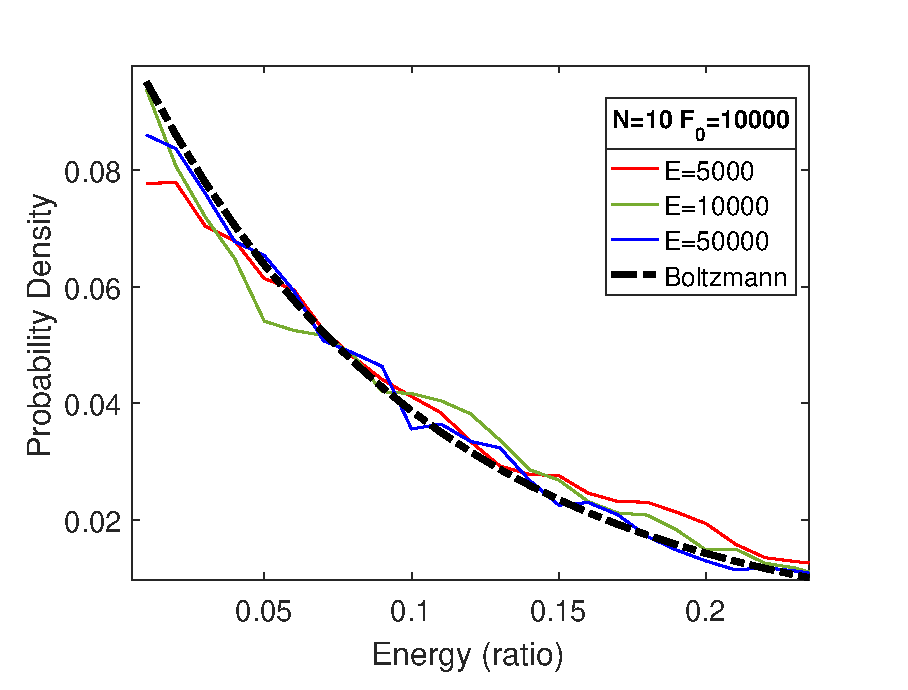
\includegraphics[scale=0.5]{ZhiyuPictures/boltzmann_N=10_F=10000_pre_rev.eps}
\caption{Energy distribution, N=10, F0=10000}
\label{fig:thermalization9}

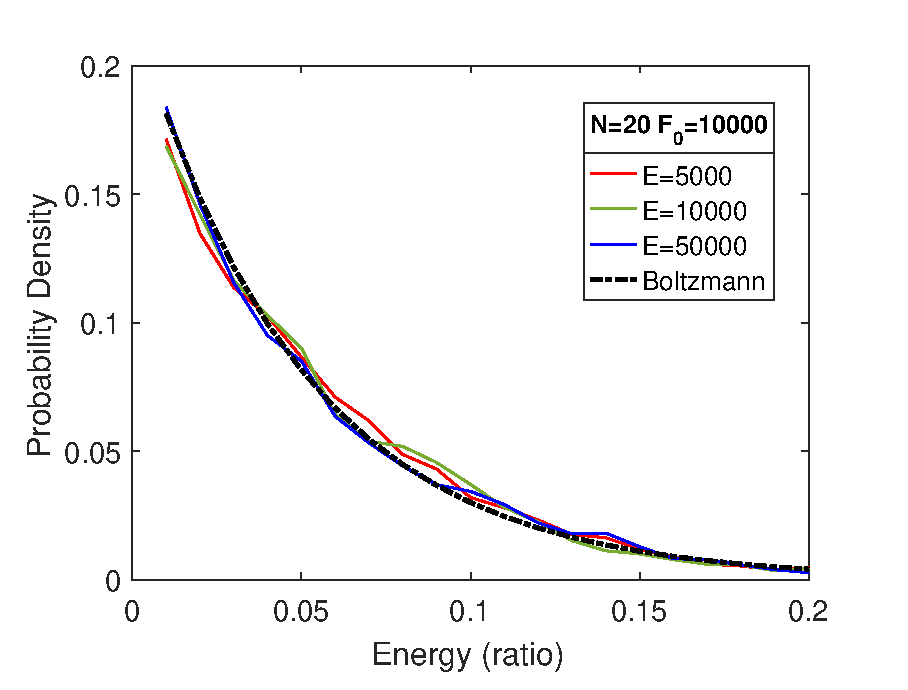
\includegraphics[scale=0.5]{ZhiyuPictures/boltzmann_N=20_F=10000_pre_rev.eps} 
\caption{Energy distribution, N=20, F0=10000}
\label{fig:thermalization10}
\end{figure}



To take the first one as an example, Y axis is logarithmically scaled. X axis is the ratio between single particle energy (where half of interaction is taken into account) and total energy of the system. The blue dotted line is the predicted Boltzmann distribution (normalized according to counts). Notice that normalizing of the Boltzmann line only change the intercept, leaving slope untouched, which means the slope is the only thing to compare. In  Energy ratio smaller than 30\%, the experiment (colourful curves) fits well with the prediction. When energy of a single particle is higher, one can think of the "bath" formed by the remaining part has lower temperature, thus counts decrease faster to zero than Boltzmann law.

It is evident form $Nk_BT=E$ that the slope of Boltzmann distribution in this figure only depend on N. That is the reason why we want to measure at different N below. 

In fig.\ref{fig:thermalization9} and fig.\ref{fig:thermalization10}, the curve is slightly deviated from the standard Boltzmann distribution, which is probably due to the contribution of density of states (DOS). Possibility is proportional to Boltzmann exponential factor multiplied by density of states. The reason why we did not take DOS into account previously lies in that the DOS is a constant for simple harmonic oscillator. However, for simple harmonic oscillators with short range interaction, the energy shell is deformed in the small region of $|x_i-x_j|<\sigma$ so that the DOS is no longer a constant. But since $\sigma<<R$, one can think of this as a small modification. Therefore, the tendency of the curve in fig.\ref{fig:thermalization9} and fig.\ref{fig:thermalization10} is deviated slightly from Boltzmann distribution.
 


\subsection{Relaxation in Phase-space}

When describing simple harmonic motion, it is usually convenient to use the language of phase-space (of single particle). In the phase-space, the motion becomes circular, so each of these particles has two independent degree of freedom, i.e., modulus and phase angle. Here, independent means that the simple harmonic oscillation never ``mix" these two degrees of freedom. In view of this, when it comes to ``thermalization", one may notice that the thermalization of energy, which is just the modulus, does not ensure the thermalization of phase angle. To distinguish these two kind of meanings of ``thermalization", we will call the process of energy distribution going to equilibrium ``thermalization", while the process of phase angle going to equilibrium ``relaxation". The time scale of thermalization and relaxation could be different in principle. We start with the configuration where particles' velocities are set to be zero, which means in phase-space the cloud is line shape at the beginning. If the time scale of thermalization is much longer than that of relaxation, we will see cloud going to isotropic in a short time, and radius distribution slowly evolves to Boltzmann distribution. If the relaxation time is longer than the thermalization time, the cloud will maintain elliptical shape or elliptical shape for a long time while the radius distribution is already Boltzmann.

To study the relaxation, it is convenient to go back to the picture introduced in discussing breathing frequency, since in that chapter, we focus on the average effect of collision on precession motion, but now we focus on the fluctuation near this average effect. Let's recall two distinct regime discussed in Fig.\ref{fig:Breathingfrequency3}. These two regime will show different behavior of relaxation.

In ``bouncing regime", (see Fig.\ref{fig:Breathingfrequency3}(a))particles' position in phase-space have a finite shift $\sim\sigma$ in one collision. As is discussed in former chapter, the average effect of this shift result in precession motion in phase-space and lead to a perturbed breathing frequency. This result is based on approximating the mean effect of collision process with the collision between two particles aligned symmetrically on P axis. However, in reality, the particles 
are everywhere so that the shift do not rotate the particles' phase angle by the same amount in every collision, thus the increase of the phase angle of each particle can be thought of as a wide distribution with a non-zero mean value. As a result of this distribution, the phase angle soon got thermalized, which means the ``relaxation time" is short.

In `` passing regime", (see Fig.\ref{fig:Breathingfrequency3}(b)),the maximal shift of position in phase-space starts to decrease with the decrease of $F_0$. The shift $\delta$ decrease as $\delta\sim F_0^2$. This means the particles are localized in their original position when $F_0$ is smaller-- it is natural to get this conclusion, since the weaker the interaction is, the longer time it takes to ``relax".

All our discussion before is based on the approximation that every particle collide with each other once in one period. But this is hardly true in reality. If the number of collision in every period is taken into account, these two regime looks even more different: In ``bouncing regime", the average precession speed is significant, (see Fig.\ref{fig:Breathingfrequency4}), which means each collision cause a finite precession. The fluctuation of the number of collision one particle has in each period will contribute to the divergence of their phase angles. On the contrary, in ``passing regime", (see Fig.\ref{fig:Breathingfrequency4}), the breathing frequency is close to 2, which means the average effect of collision create zero precession speed. As a result, even though the number of collision is not a constant, it has on average no effect whether one particle collide more or less in one period. 

To directly check this argument, we can inspect the frequency spectrum of $R(t)$. As is shown in FIG.\ref{fig:frequencyspectrum}, when $F_0$ is very small (red curve), the peak is very sharp and peak frequency is exactly 2. When $F_0$ goes far beyond the threshold value of $\frac{E}{N\sigma}$ (blue, purple, pink, etc.), the peak becomes a wide distribution with a peak value deviated far from 2, which lead to  fast thermalization according to our argument before.

\begin{figure}[hbtp]
\centering
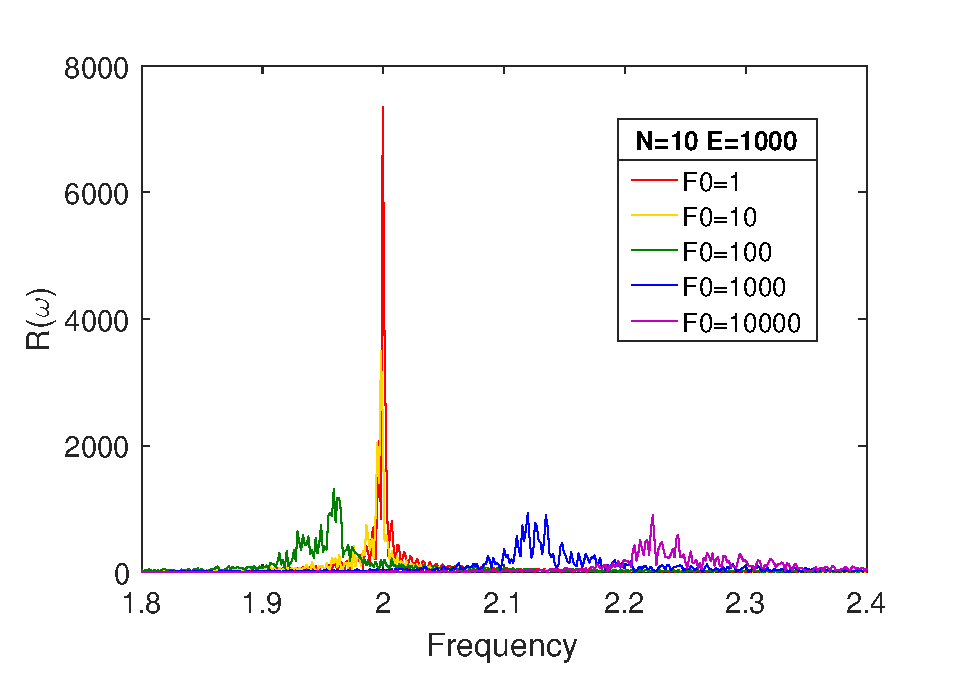
\includegraphics[scale=0.5]{ZhiyuPictures/freq_spectrum_N=10_E=1000_pre_rev.eps}
\caption{Frequency spectrum, measured over $10^4$ time units.\label{fig:frequencyspectrum}}
\end{figure}

\subsection{Lyapunov Exponents}
To see the time scale of ``thermalization" and ``relaxation" more systematically, we may measure the Lyapunov Exponents. Lyapunov Exponents(LE) describes how fast one orbit diverge from its nearby orbits in phase-space. But for high dimensional system, LE is a spectrum that manifest the instability of the trajectory along each direction. The largest Lyapunov exponents (LLE) reflects the time scale that system lose its memory in phase-space. We will measure the LLEs along our trajectory and plot its distribution.

\begin{figure}[hbtp]
\centering
%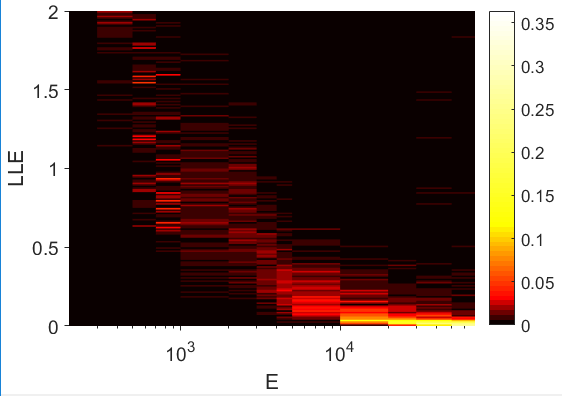
\includegraphics[scale=0.4]{ZhiyuPictures/LLEdistribution_1_11_pre_hot1_screenshot.png}
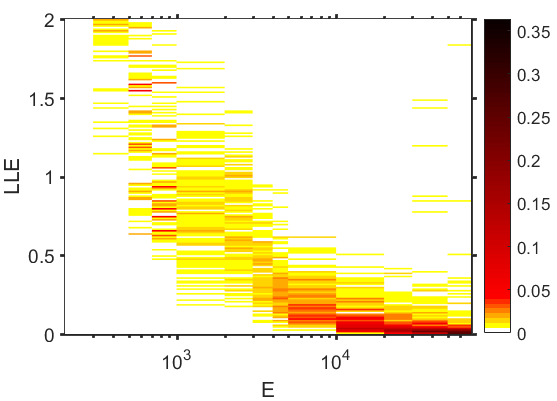
\includegraphics[scale=0.4]{ZhiyuPictures/LLEdistribution_1_11_pre_hot2_screenshot.png}
\caption{LLE distribution for N=5, F0=1000, scan E.``hot"(reversed)}\label{fig:LLEdistribution1}
\end{figure}

%\begin{figure}[hbtp]
%\centering
%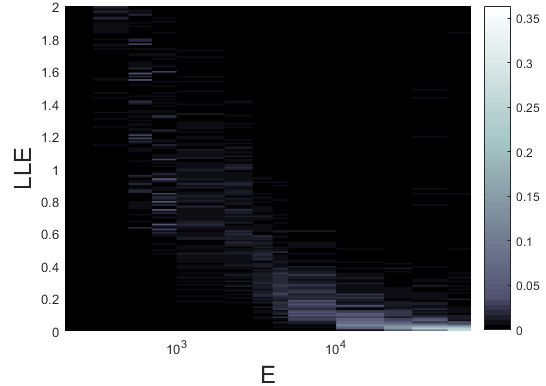
\includegraphics[scale=0.4]{ZhiyuPictures/LLEdistribution_1_11_pre_bone1_screenshot.png}
%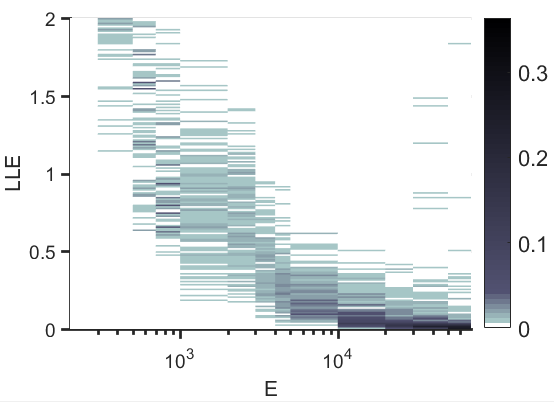
\includegraphics[scale=0.4]{ZhiyuPictures/LLEdistribution_1_11_pre_bone2_screenshot.png}
%\caption{``bone". top(bottom):modified(reversed)}
%\end{figure}


fig.\ref{fig:LLEdistribution1} shows the distribution of LLE by color. The LLE decrease with the growth of Energy. The crucial part is near E=5000. The most probable value of LLE goes down from 1 to 0.1,which indicate that \textbf{the shortest time scale becomes longer than an oscillation period when E is larger than 5000}. And E=5000 is exactly our prediction value of thermalization threshold. So there is a correspondence between energy thermalization and LLE. 
The size of bin(resolution of LLE) in fig.\ref{fig:LLEdistribution1} is 0.01, so when E goes far beyond the thermalization threshold, the LLE distribution is not that clear. We only know that LLE is concentrated close to zero in high E regime.




\subsection{{\color{red}{Shape of Distribution in Phase-space}}}
%To date, we have verified that the energy distribution will go to Boltzmann distribution. However, even if a system have reached Boltzmann distribution, it doesn't mean that the system has completely ``forgotten" its initial state. There is other information that could still exist, for instance, the shape of distribution cloud in phase-space. One of the reasons why we care about this quantity is that it has a strong effect on breathing behavior. For instance, if the distribution cloud is a thin ellipse (all particles oscillate in phase), the amplitude of oscillation of the cloud radius will be very large. On the contrary, if the cloud is a circle (particles phase of oscillation are completely random), we will not see oscillation at all. Going to equilibrium not only require the thermalization mentioned in last section, but also require reaching a stable configuration in phase-space distribution (relaxation).

If the oscillating phases of particles are highly correlated, for example, initial state with zero velocity, the shape of cloud will be a thin ellipse. If the phase of oscillation is completely random, the cloud should be isotropic in phase space. In view of this, we defined a shape factor S:
\\$S=\frac{a-b}{a+b}$, where a and b are long axis and short axis of inertia ellipse in phase space respectively. a,b can be calculated by diagonalizing the inertia matrices I: $I_{xx}=\sum{x^2}, I_{xp}=I_{px}=\sum{xp},I_{pp}=\sum{p^2}$
S=1 for line-shape distribution, S=0 for circular distribution.
The time evolution of S will probably show how fast the distribution ``forget" its initial shape.  


\section{Conclusion}
We studied the nonequilibrium property of one-dimensional classical gas with finite range repulsive interaction. We first studied the relation between breathing mode frequency and interaction parameter as well as total energy. We found the breathing frequency could be estimated by \ref{eq:breathingfrequency1}. And the mechanism behind this relation is that the momentum transfer which happens instantly in collision saves the particles some time from traveling this distance. So the physics is completely the same as hardcore particle.
We found that the thermalization behavior is controlled by the competition between the interaction strength and the average energy. We point out that there could be two independent time scales in simple harmonic system in principle. One of them corresponds to the relaxation time of the energy distribution. The other one corresponds to the relaxation time of the angular distribution in phase space, which will determine the decay rate of the amplitude of the breathing mode. However, with the form of interaction we used, i.e. finite range constant repulsive force, we found those two time scales diverge only when interaction vanish, which is a trivial singular point. In addition, the relaxation behavior of the angular distribution and radial distribution in phase space are similar. We attribute it to the fact that there is no essential bias between angular and radial transfer in phase-space for this simple form of interaction. The longest time scale is verified numerically by Largest Lyapunov Exponent. A further question could be asked is whether there is a subtle form of interaction that could give those two time scales essentially different behavior. The observation of two different time scales in one system would be interesting.



\begin{comment}
\section{others(those I haven't organized it into the text in logical order but may be useful)}

\subsection{Evolution of $R(t)$ and $\sqrt{\delta^2R(t)}/R(t)$} 
Results are shown in fig.\ref{fig:others1}

\begin{figure}[hbtp]

\centering
\includegraphics[scale=0.3]{D:/matlab2016/MolecularDynamics/figure/fluc_of_R_with_time2.eps}
\caption{fluctuation of R with time }
sigma=0.01(short range), $F_0=0.1(black), 1(blue), 10(green) ,100(red)$
\label{fig:others1}
\end{figure}


\subsection{Detailed discussion of two-particle motion}
{\color{red}{This chapter previously follow the subsection ``two-particle case" in subsection ``Dynamics study" in section ``Thermalization". But then I found we haven't used these result. So I put it at the end for the time being}}.
  

From now on, let's stand in the the frame of center of mass to observe the motion of two-particle system. In this frame, without interaction, we will find two particles sitting symmetrically in an equivalent harmonic trap (black curve), whose shape is identical to the trap we see in the static frame. As a result, there frequency of relative motion is exactly $2\omega$(since two particle are identical). We label the position of center of mass as 0. And we may only analyze the motion on positive axis since positive and negative are symmetric. 

Now, let's consider the interaction between them. Because of interaction, the potential curve between $+-\frac{\sigma}{2}$ should be modified to another parabolic curve that simultaneously satisfies the following two condition:\\
1) intersect with black curve at $+-\frac{\sigma}{2}$\\
2) minima is $+-\frac{F_0}{m\omega_0^2}$, which comes from a simple harmonic oscillator with an extra constant force $F_0$\\
Thus, it is obvious that by comparing $\frac{F_0}{m\omega_0^2}$ and $\sigma$, we can at least divide our parameter into several regime:\\
1) When $\frac{F_0}{m\omega_0^2\sigma}>0.5$, we will have the blue curve (see figure \ref{fig:thermalization2})\\
2) When $\frac{F_0}{m\omega_0^2\sigma}<0.5$, the red curve\\
3) When $\frac{F_0}{m\omega_0^2\sigma}=0.5$, the green one.\\
For those three types of curve, the significant difference is only at low energy case:\\
For the red one, particle will oscillate at constant frequency $\omega$;
For the blue one, when energy is lower, since the first derivative of the curve in the neighbourhood is non-zero, the frequency goes to infinity;
For the green curve, in low energy limit, it takes finite time to finish half period of oscillation, while infinitesimal time is spent on the slope part. Thus, frequency will converge to  $2\omega$.

\begin{figure}
\subfigure[]{
\begin{minipage}[b]{0.3\textwidth}
\includegraphics[scale=0.17]{ZhiyuPictures/freq_scanE_1.png} 
\end{minipage}
}
\subfigure[]{
\begin{minipage}[b]{0.3\textwidth}
\includegraphics[scale=0.17]{ZhiyuPictures/freq_scanE_2.png} 
\end{minipage}
}
\subfigure[]{
\begin{minipage}[b]{0.3\textwidth}
\includegraphics[scale=0.17]{ZhiyuPictures/freq_scanE_3.png} 
\end{minipage}
}
\centering
\caption{Frequency of relative motion with internal energy in three regime} Numbers in the legend is the value of $\frac{F_0}{m\omega_0^2\sigma}$
\label{fig:thermalization3}
\end{figure}
\end{comment}

\bibliography{mybib}
 
 \end{document}
